% To-dos
% - See comments labeled "TODO" below
% - Say why we use the low-alpha sequence
%   - Very old stars are bad because gradients flatten, very young stars are bad
%     because they are clumpy
% - Good ages could be used as a tag
% - What assumptions do we *not* have to make
%   - Separability
% - Audit abstract for discussion of phase-mixing and time invariance
%   - Equilibrium assumption is Hard
% - Note that we compare to RC-only sample and don't see any major differences
% - Cite Bland-Hawthorn to note that all solar z positions are ~20–30 pc

% Send it to:
% - Glenn Van de Ven -- Schwarzschild models of external galaxies
% - Bovy, Sanders, Das, Binney, Tremaine -- extended DF types
%

% style guide
% -----------
% - They are abundance RATIOs not abundances.
% - Is it our sample or our stars or what? "the parent sample"
% - We need a "name" for our smooth sine-and-cosine fits (blue curves).
%   "Fourier expansion model"?

\documentclass[modern]{aastex63}

\usepackage{xcolor}
\usepackage{amsmath}

\newcommand{\documentname}{\textsl{Article}}
\newcommand{\sectionname}{Section}
\renewcommand{\figurename}{Figure}
\newcommand{\equationname}{Equation}
\renewcommand{\tablename}{Table}

% Misc.
\newcommand{\bs}[1]{\boldsymbol{#1}}

% Missions
\newcommand{\project}[1]{\textsl{#1}}

% Packages / projects / programming
\newcommand{\package}[1]{\textsl{#1}}
\newcommand{\acronym}[1]{{\small{#1}}}
\newcommand{\github}{\package{GitHub}}
\newcommand{\python}{\package{Python}}

% Stats / probability
\newcommand{\given}{\,|\,}
\newcommand{\norm}{\mathcal{N}}
\newcommand{\pdf}{\textsl{pdf}}

% Maths
\newcommand{\dd}{\mathrm{d}}
\newcommand{\TT}[1]{\ensuremath{{#1}^{\mathsf{T}}}}
\newcommand{\transp}{\ensuremath{^{\mathsf{T}}}}
\newcommand{\inv}[1]{{#1}^{-1}}
\newcommand{\argmin}{\operatornamewithlimits{argmin}}
\newcommand{\mean}[1]{\left\langle #1 \right\rangle}

% Non-scalar variables
\renewcommand{\vec}[1]{\ensuremath{\bs{#1}}}
\newcommand{\mat}[1]{\ensuremath{\mathbf{#1}}}

% Unit shortcuts
\newcommand{\Msun}{\ensuremath{\mathrm{M}_\odot}}
\newcommand{\Mjup}{\ensuremath{\mathrm{M}_{\mathrm{J}}}}
\newcommand{\kms}{\ensuremath{\mathrm{km}~\mathrm{s}^{-1}}}
\newcommand{\mps}{\ensuremath{\mathrm{m}~\mathrm{s}^{-1}}}
\newcommand{\pc}{\ensuremath{\mathrm{pc}}}
\newcommand{\kpc}{\ensuremath{\mathrm{kpc}}}
\newcommand{\kmskpc}{\ensuremath{\mathrm{km}~\mathrm{s}^{-1}~\mathrm{kpc}^{-1}}}
\newcommand{\dayd}{\ensuremath{\mathrm{d}}}
\newcommand{\yr}{\ensuremath{\mathrm{yr}}}
\newcommand{\AU}{\ensuremath{\mathrm{AU}}}
\newcommand{\Kel}{\ensuremath{\mathrm{K}}}
\newcommand{\mas}{\ensuremath{\mathrm{mas}}}

% Astronomy
\newcommand{\DM}{{\rm DM}}
\newcommand{\abunratio}[2]{\ensuremath{{[\mathrm{#1}/\mathrm{#2}]}}}
\newcommand{\feh}{\abunratio{Fe}{H}}
\newcommand{\mh}{\abunratio{M}{H}}
\newcommand{\alphafe}{\abunratio{\alpha}{Fe}}
\newcommand{\mgfe}{\abunratio{Mg}{Fe}}
\newcommand{\df}{\acronym{DF}}
\newcommand{\logg}{\ensuremath{\log g}}
\newcommand{\Teff}{\ensuremath{T_{\textrm{eff}}}}
\newcommand{\mtwomin}{\ensuremath{M_{2, {\rm min}}}}

% Colors:
\definecolor{tabblue}{HTML}{4E79A7}
\definecolor{taborange}{HTML}{F28E2B}
\definecolor{tabgreen}{HTML}{59A14F}
\definecolor{tabred}{HTML}{E15759}
\definecolor{tabpurple}{HTML}{B07AA1}

% TODO:
\newcommand{\TODO}[1]{{\color{tabgreen}\textbf{TODO:} #1}}
\newcommand{\APWTODO}[1]{{\color{tabpurple}\textbf{APW TODO:} #1}}
\newcommand{\HOGGTODO}[1]{{\color{tabred}\textbf{HOGG TODO:} #1}}


% text macros
\newcommand{\methodname}{\textsl{Chemical Torus Imaging}}
% Hogg doesn't like these names because they don't refer to the abundance tags
% Torus Tomography
%   Torus Topography (see what I did there?)
%   Torus--Tangents Topography (TTT)
%   Topographic Torus Mapping (TTM)
%   Torus--Tangent Tags Topography (TTTT)
% Orbit Imaging / Torus Imaging
%   Abundance Orbit Imaging / Abundance Torus Imaging
%   Invariant Orbit Imaging / Invariant Torus Imaging
%   Invariance Imaging
% Abundance-Moment foliation (AMF)
%   Abundance-Moment laminae (AML)
%   Abundance Isopleth Method (AIM)
% Abundance Torus Machinery (ATM)
%   Abundance Torus Method (ATM)
%   Abundance Torus Maschine (ATM)
%   Element Torus Maschine (ETM)  MAYBE RIX CAN GIVE US ONE GERMAN WORD FOR THIS
% Toroidal abundance blender (TAB)
%   Toroidal abundance mixer (or mixmaster) (TAM)
% Stationary Abundance Tori (SAT)
%   Stationary Abundance Torus Method (SATM)
% Chemical Tangent Scanning (CT Scan)
% Chemical Tangents
%   Abundance Tangent Method (ATM)
%   Compositional Tangents
% Composition Gradient Method (CGM)
% Abundance Geometry
% The Magical 3-torus of Invariance (MTI)
% Totoro
% Torus Imaging
%   Chemical Torus Imaging
%   Elemental Torus Imaging
% Chemical Torus Tracing

% Project-specific macros - all others go in preamble.tex
\newcommand{\gaia}{\textsl{Gaia}}
\newcommand{\dr}[1]{\acronym{DR}#1}
\newcommand{\apogee}{\acronym{APOGEE}}
\newcommand{\sdss}{\acronym{SDSS}}
\newcommand{\sdssiv}{\acronym{SDSS-IV}}
\newcommand{\sdssv}{\acronym{SDSS-V}}
\newcommand{\galah}{\acronym{GALAH}}
\newcommand{\hermes}{\acronym{HERMES}}
\newcommand{\nstars}{56,324}

\newcommand{\mdisk}{\ensuremath{\mathrm{M}_\mathrm{disk}}}
\newcommand{\mratio}{\ensuremath{\mdisk / \mdisk^\star}}

\newcommand{\TODO}[1]{{\color{tabgreen}\textbf{TODO:} #1}}
\newcommand{\APWTODO}[1]{{\color{tabpurple}\textbf{APW TODO:} #1}}
\newcommand{\HOGGTODO}[1]{{\color{tabred}\textbf{HOGG TODO:} #1}}


% trust in Hogg
\setlength{\parindent}{1.1\baselineskip}
\renewcommand{\twocolumngrid}{}
\sloppy\sloppypar\raggedbottom\frenchspacing
\renewcommand{\doi}[1]{{\footnotesize\href{https://doi.org/#1}{#1}}}

\shorttitle{geometry of abundances and orbits}
\shortauthors{price-whelan, hogg, et al.}

\begin{document}
\graphicspath{ {figures/} }
\DeclareGraphicsExtensions{.pdf,.eps,.png}

\title{\textbf{%
    \methodname: \\
    Using element abundances to map orbits and mass in the Milky Way
    }}
    % Revealing the orbital foliation of phase space\\
    % through invariances of element-abundance distributions

\newcommand{\affcca}{Center for Computational Astrophysics, Flatiron Institute, 162 Fifth Ave, New York, NY 10010, USA}
\newcommand{\affccpp}{Center for Cosmology and Particle Physics, Department of Physics, New York University, 726 Broadway, New York, NY 10003, USA}
\newcommand{\affmpia}{Max-Planck-Institut f\"ur Astronomie, K\"onigstuhl 17, D-69117 Heidelberg, Germany}
\newcommand{\affcolumbia}{Department of Astronomy, Columbia University, New York, NY 10027, USA}

\author[0000-0003-0872-7098]{Adrian~M.~Price-Whelan}
\affiliation{\affcca}

\author[0000-0003-2866-9403]{David~W.~Hogg}
\affiliation{\affcca}
\affiliation{\affmpia}
\affiliation{\affccpp}

\author[0000-0001-6244-6727]{Kathryn~V.~Johnston}
\affiliation{\affcca}
\affiliation{\affcolumbia}

\author{Melissa~K.~Ness}
\affiliation{\affcolumbia}
% \affiliation{\affcca}

\author[0000-0003-4996-9069]{Hans-Walter~Rix}
\affiliation{\affmpia}

\author{APOGEE authors}


\begin{abstract}\noindent
  The dynamics of stars in the Milky Way and nearby galaxies is often
  interpreted in an approximation where the gravitational potential is treated
  as simple and integrable and the distribution function time-invariant.
  Under these conditions, Jeans modeling---which relies on computing and
  observing moments of the distribution function---is a standard methodology for
  measuring properties of the mass distribution or potential.
  However, contemporary and near-future spectroscopic surveys measure more than
  just kinematics for huge samples of individual stars within the Milky Way and
  Local Group.
  Here we present an approach for dynamical
  inference---\methodname---that makes use of kinematic measurements
  and stellar tags (e.g., element abundance ratios, stellar ages, or other
  invariant stellar properties).
  The method exploits the fact that there are generically gradients of stellar
  tags on orbital actions (or position and velocity) in the Galaxy, and in
  steady state the distributions of any tags must be invariant with respect to
  time-variable conjugate angles.
  Thus, level sets in moments of the tag distributions must coincide with
  the orbital foliation of phase space!
  We discuss how both classical-statistics and Bayesian forward-modeling methods
  can be built on this idea, and we perform a demonstration with red giant
  stars from the \apogee\ surveys:
  We look at the vertical orbit structure in the Milky Way disk, using mean
  abundances to constrain the local disk mass (the disk--halo trade-off at fixed
  circular velocity).
  % TODO: audit this statement
  We find that the disk mass can be constrained (na\"ively) at the $<3$-percent
  level with this new method using only six element abundance ratios,
  demonstrating the promise of combining stellar tags with dynamical invariants.
\end{abstract}

\keywords{\raggedright % now from the UAT, not the AAS keyword system
  astrometry
  ---
  astrostatistics
  ---
  chemical~abundances % UGH ELEMENTS
  ---
  galaxy~dynamics
  ---
  Milky~Way~dynamics
  ---
  radial~velocity
  ---
  spectroscopy
  ---
  stellar~kinematics
  ---
  surveys
}

% \section*{}\clearpage
\section{Introduction}
\label{sec:intro}

% TODO: work in comments about Sanders/Das EDF stuff

A significant goal of modern physics and astronomy is to understand the detailed
properties of dark matter on astrophysical scales as a way of informing
constraints on its fundamental nature \citep[see, e.g., recent reviews
by][]{Bullock:2017, Buckley:2018}.
Significant effort has therefore gone into developing and applying tools for
constraining the mass distributions (i.e., dark matter distributions) of Local
Group galaxies using only kinematic observations of tracers (i.e., stars;
\citealt{Jeans, Binney:2008, somanythings}).
This challenge---using observations of tracer objects to constrain the
underlying force law---is conceptually similar to a much older problem faced by
physicists of the 17th century, who worked out that the gravitational force law
in the Solar System is proportional to the inverse square of the distance from
the Sun \citep{Newton:1687}.
That inference was based on observations that showed that orbits in the Solar
System are closed ellipses, with the Sun at one focus \citep{Kepler:1609}---that
is, they made use of observations of a few tracers (the planets) at many orbital
phases.

In our current efforts to map dark matter, we are instead in a regime where we
observe \emph{many} tracers (stars) but have little or no information about
orbital phase: We observe only a single snapshot (in time) of the stellar
orbits!
The closest we come to seeing orbits directly in the Milky Way is in the study
of stellar streams \citep[e.g.,][]{peoples}, which almost directly encode
(differential) phase information about the orbit of their progenitor systems.
But stellar streams are relatively sparse, and orbits in the Galaxy have more
degrees of freedom than orbits around a point-mass, meaning that we need many
more orbits to span the phase-space and obtain precise constraints on the mass
distribution.
One could argue then that our current task is much harder than Newton and Kepler
had it:
We seek to constrain the global distribution of dark matter around a galaxy---a
time-evolving mass distribution with nontrivial shape and radial
distribution---with only a snapshot of the tracer kinematics (and often only a
subset of phase-space dimensions).

The tools we use to constrain the Galactic force field (i.e., the dark matter
distribution) given only a snapshot of the dynamics are therefore (necessarily)
statistical in nature and do not depend on knowing the orbits of individual
stars.
Instead, these methods typically rely critically on strong assumptions about the
stationarity of the distribution of tracer orbital properties (i.e., a
``steady-state'' or ``equilibrium'' assumption) and the integrability of the
underlying gravitational potential \citep[see, e.g.,][for a review of such
methods as applied to the problem of determining the local dark matter
density]{Read:2014}.
When applied in real-world contexts on stars in the Milky Way or dwarf
spheroidal galaxies, these methods often also require further assumptions, such
as separability of the \acronym{DF}, or the velocity anisotropy profile, or
require simple parametrizations of the \acronym{DF} in order to execute these
analyses.
Generic approaches here typically require parametrized models for the
\acronym{DF} and for the gravitational force field or mass distribution
\citep[e.g.,][]{McMillan:2013, Magorrian:2014, Binney:2014, Magorrian:2019}, but
become computationally prohibitive for large data sets or flexible model forms.

For simplicity and computational efficiency, one of the most ubiquitous
approaches used for dynamical inferences is so-called ``Jeans modeling''
\citep{Binney:2008}, which use the Jeans equations to relate statistical
moments of the tracer distribution function (\acronym{DF}) to properties of the
force field.
While these methods still depend on many of the assumptions laid out above, they
have the great (computational) advantage of not having to deal with modeling the
\acronym{DF} directly.
Jeans modeling (or related analyses) have therefore been used in many
applications:
For example, to derive constraints on the local dark matter density using the
vertical ($z$--$v_z$) kinematics of stars in the solar neighborhood
\citep[e.g.,][]{Jeans:1922, Oort:1932, Bahcall:1984, Buch:2019}, the radial
profile of the Milky Way halo \citep[e.g.,][]{Watkins:2010, Zhai:2018}, the mass
profiles of Local Group satellites \citep[e.g.,][]{Evans:2009, Walker:2011}, and
the mass distributions in elliptical galaxies \citep[e.g.,][]{Romanowsky:2003,
Mamon:2005, Sonnenfeld:2012}, amongst other applications.

A contemporary ``challenge'' to applying these methods on modern data
(especially within the Milky Way) is that stellar kinematic data is now very
precise, and the phase-space is well sampled.
For example, data release (\dr{2}) from the \gaia\ mission
\citep{Gaia-Collaboration:2016, Gaia-Collaboration:2018} has provided full
phase-space kinematics (for a subset of stellar tracers) over a region several
kiloparsecs in size around the Sun.
These data have revealed evidence of dynamical disequilibrium throughout the
Galactic disk and halo \citep{Antoja:2018, Myeong:2018, Koppelman:2018,
Eilers:2020}.
Standard methods for estimating dark matter properties using stellar kinematics
therefore rely on a list of assumptions about dynamical equilibrium, symmetries,
or separability that we now know are strongly violated in the real universe and
Galaxy!
The fact that we still use and apply these methods is a reflection of the fact
that relaxing these assumptions make dynamical inferences \emph{far} more
challenging and computationally expensive.
For example, there are therefore no standard methods (e.g., analogies to Jeans
modeling) when the assumption of dynamical equilibrium is relaxed.

One reason to remain hopeful in our goal (precisely constraining the dark
matter) is that, unlike Kepler and Newton, we have excellent working models of
stars and access to much more information per star than kinematics alone.
For example, spectroscopic surveys have measured the stellar parameters and
element abundances of hundreds of thousands, and soon to be millions, of stars
\citep[e.g.,][]{DR16, Martell:2017, Deng:2012} over large regions of the
Galactic disk and halo.
It is therefore promising to think that utilizing stellar ``tags'' (element
abundances, stellar ages, or other invariant stellar properties) within
dynamical inferences will provide additional information that may help interpret
or model the Galaxy \citep[see, e.g.,][for recent methods that begin to move in
this direction, within the context of equilibrium models]{Sanders:2015,
Das:2016, Binney:2016, Iorio:2020}.

In this \documentname, we are going to demonstrate that stellar surface
abundances can be used to illuminate the orbit structure in the Milky Way, and
are therefore extremely valuable for dynamics.
In our current methodology, like all other dynamical inferences, we will work
only under strong assumptions, so we are still in the business of revealing the
orbits indirectly.
However, our approach is novel and there are many regimes in which it will be
more precise, and require fewer assumptions, than any other method.
\TODO{Expand out again, make sure to emphasize how general this idea is?}


\section{Methodological Generalities}
\label{sec:generalities}

In a well-mixed, equilibrium population, stars are in a kinematic steady state:
As time goes on, stars move along their orbits, but they do not change their
dynamical invariants (e.g., actions).
In such situations, every location in angle (the coordinates conjugate to
actions) is equally likely, or equally probably populated in any snapshot.
The ``chemical tagging'' insight \citep{Freeman:2002} is that most stars also
preserve their surface element abundances (and other stellar tags) as they
orbit, over many Galactic orbital timescales.
That is, in an integrable galaxy---a galaxy whose stellar orbits are associated
with three invariant actions---the element abundances and the dynamical actions
have something in common: They are invariant with time.
Only the conjugate angle coordinates are time-dependent.
This means that, for a well-mixed population, the detailed element abundances
can only be a function of actions, and never a function of conjugate angles.
That is a remarkably informative constraint on the configuration of the Milky
Way in the space of positions (dimensionality 3), velocities (3), and
detailed abundances (10--30, depending on the spectroscopic survey).

Consider a collection of stars (localized, say, in phase space) for which we
have measured $D$ element abundances.
This collection of stars will in general have a diversity of element abundances:
Their abundances are drawn from some distribution in $D$-dimensional
element-abundance space.
In general, the abundance distribution will depend on position in phase-space:
For example, there are observed radial and vertical abundance gradients in the
Galactic disk \citep{people}.
However, any changes we observe in these element-abundance distributions with
respect to phase-space coordinates (i.e., the six-gradient) must not project
onto the directions of increasing (or decreasing) conjugate angles in phase
space.
All gradients with respect to phase-space coordinates of the element-abundance
distribution must be orthogonal to the directions of increase (or decrease) of
the conjugate angles, and lie in the subspace of the directions of increase (or
decrease) of the dynamical actions.
The trajectories of stars in the phase space (the dynamical tori) must therefore
lie along or describe level surfaces in the element-abundance distribution!

In this \documentname, we demonstrate the utility of these gradients and
relations between element abundances and dynamical invariants in the context of
dynamical inferences in the Milky Way.
We consider stars in our Galaxy because here we can measure six-dimensional
kinematics and element-abundances for individual stars, enabling relatively
simple demonstrations of the concepts here.
However, we note that a generative model built on these concepts would, in
principle, be applicable in more general scenarios, such as for stars in Local
Group satellite galaxies where only a subset of phase-space coordinates are
measured.


\section{Data}
\label{sec:data}

% Notebook: figures/APOGEE-sample.ipynb
\begin{figure}[!tp]
  \begin{center}
  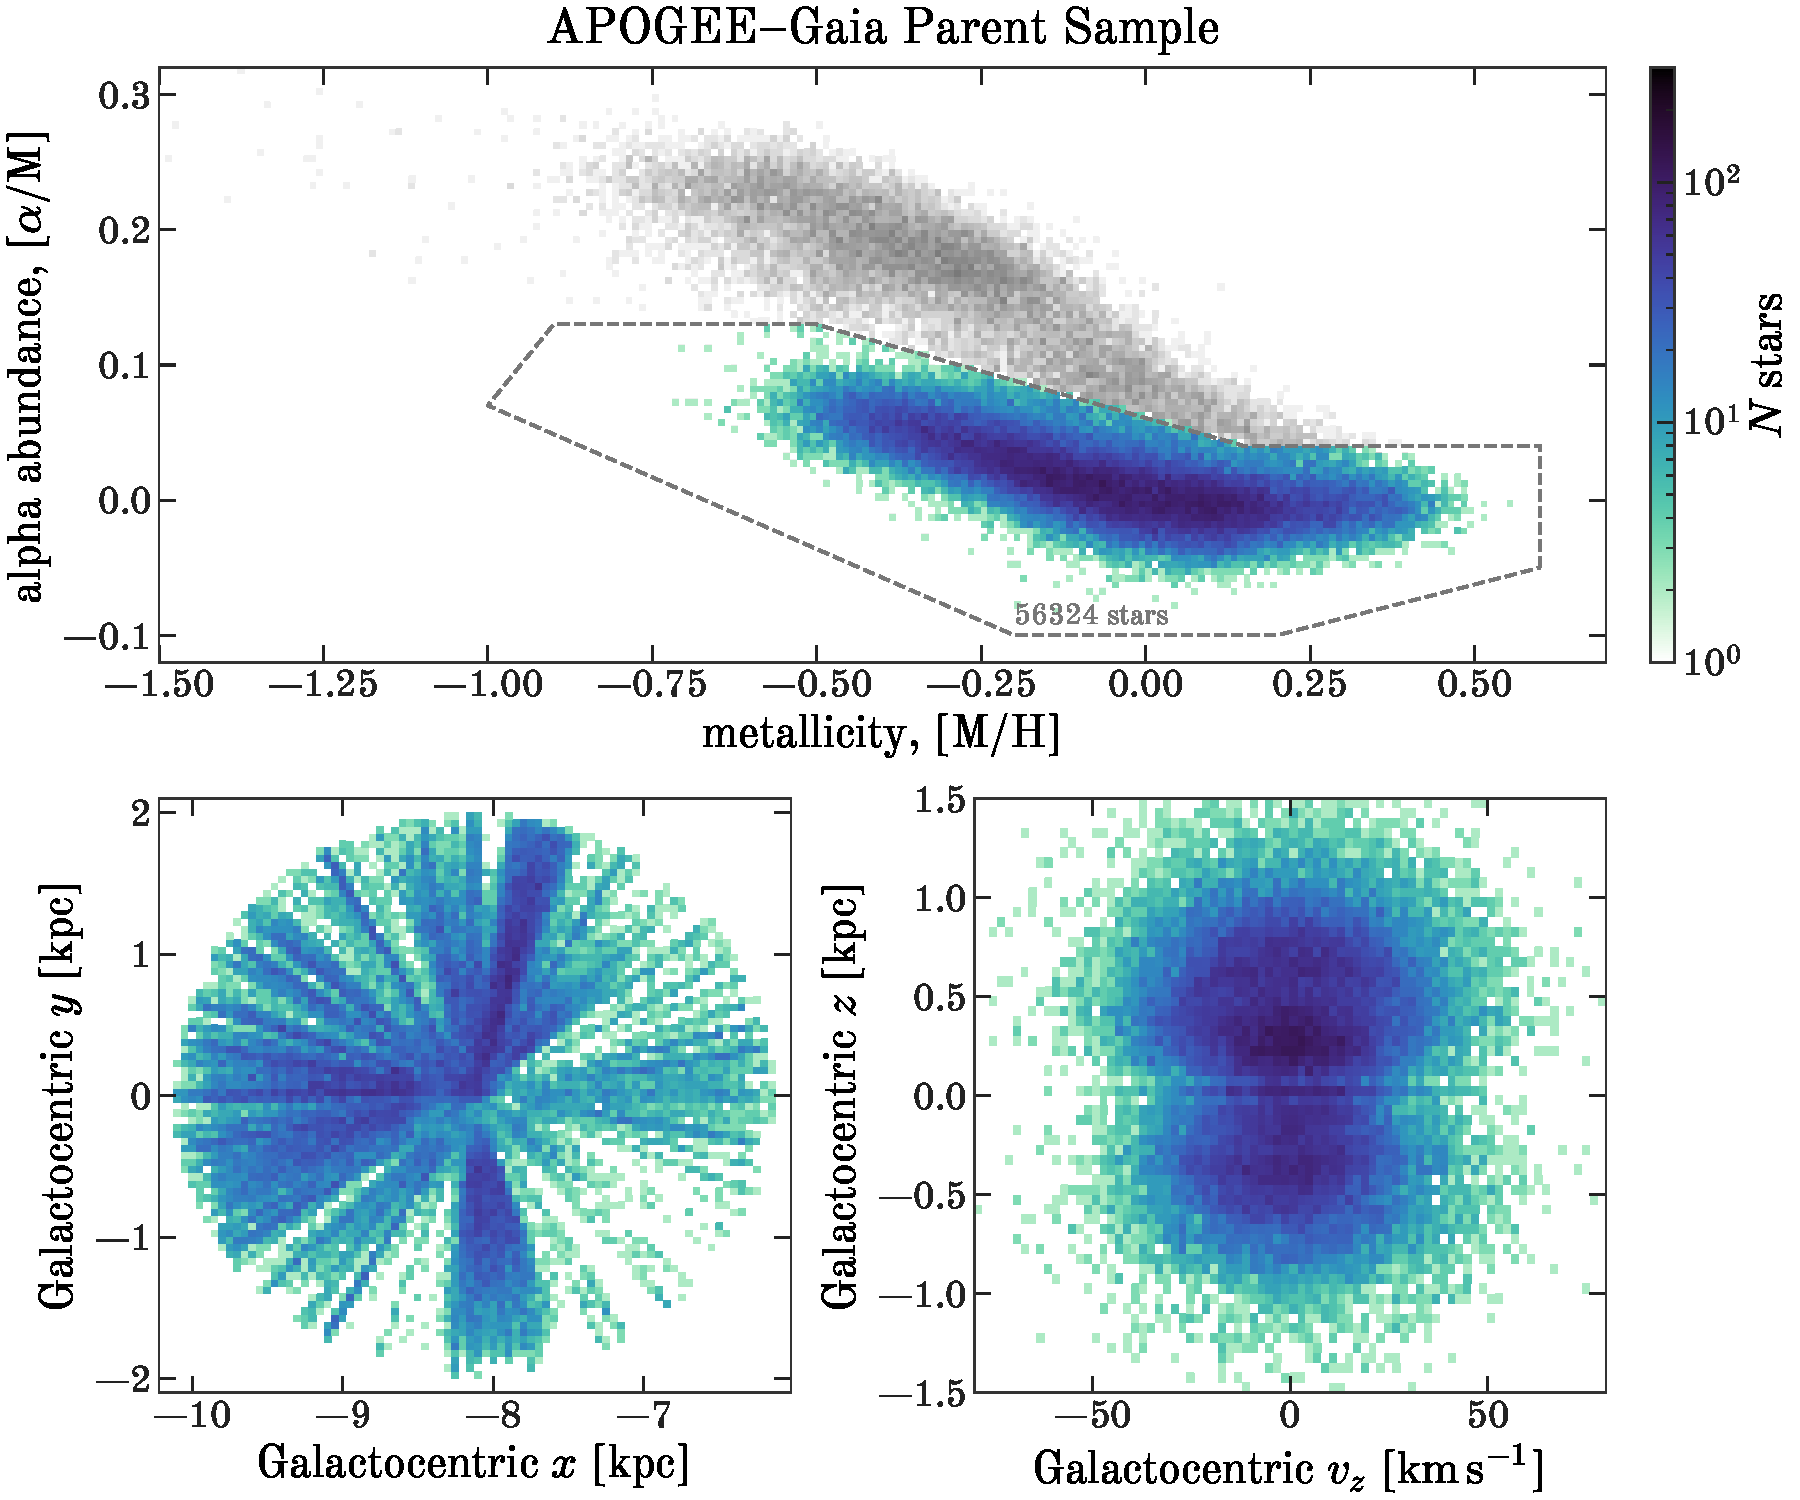
\includegraphics[width=\textwidth]{apogee-rgb-loalpha-mh-am-xy.pdf}
  \end{center}
  \caption{%
    The data sample used in this project.
    Each panel shows a 2D histogram of the stars.
    \textsl{Top panel:}
    Bulk abundance ratios measured by \apogee\ and a selection boundary (dashed
    line) used to exclude the ``high-alpha'' stars that are generally older and
    kinematically hotter.
    \textsl{Lower left panel:}
    Positions of the stars in the parent sample projected onto the Galactic
    plane, showing the spherical spatial cut and highly non-uniform (\apogee)
    spatial selection.
    Heliocentric distances to the stars are obtained by na\"ively inverting
    their \gaia\ parallax measurements.
    \textsl{Lower right panel:}
    The distributions of stars in the parent sample in vertical $z, v_z$ phase
    space.
    This panel shows that the sample is less populated at low $z$ (mainly
    because of the \apogee\ selection function), which in turn shows that the
    sample is less populated at certain values of vertical angle, $\theta_z$.
    The methods presented in this paper do not require that all angles are
    equally populated in the sample.
    \label{fig:mh-am-xy}
    }
\end{figure}

In our toy demonstrations below, our main data source is a cross-match between
spectroscopic data from the \apogee\ surveys \citep{Majewski:2017} and
astrometric data from the \gaia\ mission \citep{Gaia-Collaboration:2016,
Gaia-Collaboration:2018}.

\apogee\ is a spectroscopic sub-survey and component of the Sloan Digital Sky
Survey IV (\sdssiv; \citealt{Blanton:2017}) whose main goal is to map
the chemical and dynamical properties of stars across the Milky Way disk.
The survey uses two nearly identical, high-resolution ($R \sim 22,500$;
\citealt{Wilson:2019}), infrared ($H$-band) spectrographs---one in the Northern
hemisphere at Apache Point Observatory (APO) using the SDSS 2.5m telescope
\citep{Gunn:2006}, and one in the Southern hemisphere at Las Campanas
Observatory (LCO) using the 2.5m du Pont telescope \citep{Bowen:1973}.
The primary survey targets are selected with simple color and magnitude cuts
(\citealt{Zasowski:2013, Zasowski:2017}, Santana et al. in prep., Beaton et al.
in prep.), but the sparse angular sky coverage and limited number of fibers per
field lead to a ``pencil-beam''-like sampling of the Milky Way stellar density.
\apogee\ spectra are reduced \citep{Nidever:2015} and then analyzed (i.e., to
measure stellar parameters and abundances) using the \apogee\ Stellar Parameters
and Chemical Abundance Pipeline (\acronym{ASPCAP}; \citealt{ASPCAP,
Holtzman:2018}); here we use abundance measurements from the standard \apogee\
pipeline.

Here we use a recent internal data product (which includes all data taken
through March 2020) from the \apogee\ surveys (post-\dr{16}) that includes
$\approx\%$ more stars than the publicly-available \dr{16} catalogs \citep{DR16,
Jonsson:2020}, but was reduced and processed using the same pipeline used to
produce the \dr{16} release.
This \apogee\ catalog contains calibrated element abundance measurements for 18
elements, but these have a variety of physical origins and a range of
reliabilities and measurement precisions.
For demonstrations below, we therefore focus on a subset of eight, well-measured
(log) abundance ratios selected to have varied astrophysical origins:
\abunratio{Fe}{H}, \abunratio{C}{Fe}, \abunratio{N}{Fe}, \abunratio{O}{Fe},
\abunratio{Mg}{Fe}, \abunratio{Si}{Fe}, \abunratio{Mn}{Fe}, \abunratio{Ni}{Fe}.
In some cases, we focus on just a single element abundance, \abunratio{Mg}{Fe},
which is the most precisely and accurately determined element abundance measured
with the \dr{16} pipeline \citep{Jonsson:2020}.

\gaia\ is primarily an astrometric mission and survey
\citep{Gaia-Collaboration:2016} that obtains sky position, proper motion, and
parallax measurements for $>1$ billion stars limited only by their apparent
magnitudes (\gaia\ $G \lesssim 20.7$).
Here we use parallax and proper motion measurements released in \gaia\ \dr{2}
\citep{Gaia-Collaboration:2018, Gaia-astrometric:2018}.

We cross-match the \apogee\ sample to \gaia\ \dr{2} using the \apogee-provided
\acronym{2MASS} \citep{Skrutskie:2006} identifiers, and the \gaia-provided
cross-match between \gaia\ \dr{2} and the final \acronym{2MASS} point source
catalog \citep{Gaia-crossmatch:2019}.
We then apply a number of quality cuts and other selections to limit the catalog
to chemically thin-disk, red giant branch (RGB) stars with well-measured stellar
parameters and abundances, high signal-to-noise parallax measurements, but
excluding stars targeted in stellar clusters and dwarf galaxies.
In detail, our selections include:
\begin{itemize}
  \item \acronym{ASPCAP} quality flag (\texttt{ASPCAPFLAG}) must not contain
    \texttt{STAR\_BAD} or \texttt{STAR\_WARN},
  \item $3500~\Kel < \Teff < 6500~\Kel$,
  \item $1.5 < \logg < 3.4$,
  \item combined spectroscopic signal-to-noise ${\rm SNR} > 20$,
  \item \apogee\ targeting bit flags must not indicate that the source was part
    of a special program to observe stellar clusters, dwarf galaxies, M31 stars,
    stellar streams, or moving groups; this \emph{excludes} stars with the
    following bits enabled:
    \begin{itemize}
      \item \texttt{APOGEE\_TARGET1}: (9. 18, 24, 26)
      \item \texttt{APOGEE\_TARGET2}: (10, 18)
      \item \texttt{APOGEE2\_TARGET1}: (9, 18, 20, 21, 22, 23, 24, 26)
      \item \texttt{APOGEE2\_TARGET2}: (10)
      \item \texttt{APOGEE2\_TARGET3}: (5, 14, 15)
    \end{itemize}
  \item stars are part of the ``low-alpha'' (or ``chemical thin disk'')
    population (see polygonal selection in the top panel of
    \figurename~\ref{fig:mh-am-xy}),
  \item \gaia\ parallax $\varpi > 0.5~\mas$,
  \item \gaia\ parallax signal-to-noise $\varpi / \sigma_\varpi > 8$.
\end{itemize}
The \apogee\ catalog contains a small number of duplicates (duplicated source
identifier \texttt{APOGEE\_ID}); To unique-ify our sample in these cases, we
keep only the entry with highest signal-to-noise.
The final parent sample contains \nstars\ RGB stars with high-quality \apogee\
and \gaia\ data.

For each star in the parent sample, we compute na\"ive distance estimates by
inverting the parallax, $d = 1/\varpi$.
While this is generally not a safe way of computing distance from parallaxes
(see, e.g., \citealt{Bailer-Jones:2015}), our sample stars are (by construction)
relatively nearby and have high signal-to-noise parallax measurements.
Using a parallax signal-to-noise selection has its own consequences, especially
in that it makes the sample selection function complex and non-intuitive.
However, our methodology should be relatively insensitive to selection effects,
and since the demonstrations that make use of these distance measurements below
are meant to be illustrative examples, we ignore these details in what follows.
This sample is visualized in bulk element abundance ratios and Galactocentric
positions in \figurename~\ref{fig:mh-am-xy}.


\section{Milky Way mass model and computing actions}
\label{sec:mw-model}

Our methodology and demonstrations below rely on computing actions and angles
for stars, which depend on the mass distribution of the Milky Way and the solar
position and motion with respect to a Galactocentric reference frame.

For the solar position, we use the recent precise measurement of the
Sun--Galactic center distance from the \acronym{GRAVITY} collaboration, $r_\odot
= 8.122~\kpc$ \citep{Gravity:2018}, and adopt $z_\odot = 20.8~\pc$ as the solar
height above the Galactic midplane \citep{Bennett:2019}.
In Galactocentric Cartesian coordinates, we use a right-handed coordinate system
such that the Sun is at $\bs{x}_\odot = (-8.1219, 0, 0.0208)~\kpc$ and the
solar velocity is $\bs{v}_\odot = (12.9, 245.6, 7.78)~\kms$ \citep{Drimmel:2018,
Reid:2004, Gravity:2018}.

We represent the density distribution (or gravitational potential) of the
Milky Way using an idealized, four-component mass model consisting of a
spherical Hernquist bulge \citep{Hernquist:1990}, spherical Hernquist nucleus,
an axisymmetric Miyamoto-Nagai disk \citep{Miyamoto:1975}, and a spherical
Navarro-Frenk-White dark matter halo \citep{Navarro:1996}.
Most of the parameters of these components are fixed to their default values
from the \texttt{MilkyWayPotential} class implemented in the \package{gala}
Python package \citep[v1.2;][]{gala}:
Briefly, the bulge parameters (mass and scale radius) and disk parameters (total
mass, scale height, and scale radius) are initially set to match the
\texttt{MWPotential2014} implemented in \package{galpy} \citep{Bovy:2015}, and
the dark matter halo parameters (virial mass and scale radius) are initially set
by fitting the enclosed mass profile of the mass model to a compilation of
recent enclosed mass measurements.\footnote{As described in
\url{https://gala.adrian.pw/en/latest/potential/define-milky-way-model.html}.}
However, the mass of the disk is then adjusted to match a circular velocity of
$v_{\rm circ}(R_\odot) = 229~\kms$ at the solar radius \citep{Eilers:2019}.
Our fiducial mass model therefore adopts the default \texttt{MilkyWayPotential}
parameters except for the disk mass, which is set to $\mdisk^\star = 6.526
\times 10^{10}~\Msun$.
Later in this \documentname, we vary the disk mass \mratio, but we adjust the
dark matter halo mass to keep the circular velocity at the solar radius, $v_{\rm
circ}(R_\odot)$, constant.

In a given potential model, we compute actions, $\bs{J} = (J_R, J_\phi, J_z)$,
and angles, $\bs{\theta} = (\theta_R, \theta_\phi, \theta_z)$, for a star using
the ``St\"ackel Fudge'' \citep{Binney:2012, Sanders:2012} as implemented in
\package{galpy} \citep{Bovy:2015}.
We solve for the focal length, $\Delta$, of the locally-approximating St\"ackel
potential for each star's orbit by numerically computing the orbit of each star
for four orbital periods.
In practice, for computational efficiency, we do this initially for a range of
potential models (i.e., different $\mratio$ values) and use linear interpolation
to predict the value of $\Delta$ for each orbit given a value of $\mratio$.

We assess the accuracy of using the St\"ackel Fudge for orbits with large
vertical excursions from the Galactic disk by comparing actions computed with
the St\"ackel Fudge to actions computed with a more accurate action solver.
For a set of trial orbits (meant to span the range of vertical actions we see in
our sample of \apogee\ stars) over a range of disk masses (from
$\mratio=0.5$--$1.5$), we compute actions both with the St\"ackel Fudge and with
the ``O2GF'' method defined in \citet{Sanders:2014}.
The O2GF method works by numerically integrating an orbit for a given star and
solving for the generating function to transform from actions computed in a toy
potential model to the actions in the potential model of interest (as defined in
\citealt{Sanders:2014}, and implemented in \package{gala}).\footnote{This method
is referred to as the ``O2GF method'' in \citet{Sanders:2016}.}
This method has some tuning parameters related to the total orbital integration
time and time step, and the number of Fourier components to include in the
Fourier expansion used to represent the generating function, $N_{\rm max}$.
We use an Isochrone potential as our toy potential model, set the total
integration time for each star to 128 (radial) orbital periods, $T=128\,P_r$,
and set the time step to $\Delta t = P_r / 256$. For all stars, we set $N_{\rm
max} = 8$ (following \citealt{Sanders:2016}).
We find that in all cases, the values of the actions agree to within $<10\%,
<0.1\%, <0.5\%$ for $J_R, J_\phi, J_z$, respectively, with the largest
disagreements only affecting a small fraction of the stars in our sample with
the largest excursions from the Galactic plane.

For computational efficiency, we therefore use the St\"ackel Fudge as our
primary method for computing actions in what follows.
% the three actions and angles for all stars in
% our parent sample (see \sectionname~\ref{sec:data}) in each of the 15 potential
% models with different disk-mass to halo-mass ratios (see above).
To additionally speed up computation, we typically also parallelize the
computation of the actions (over stars) using the Python package
\package{schwimmbad} \citep{schwimmbad}.


\section{Motivation from Observed Element Abundance Gradients}
\label{sec:motivation}

% Notebook: figures/APOGEE-zvz-orbits.ipynb
\begin{figure}[!tp]
  \begin{center}
  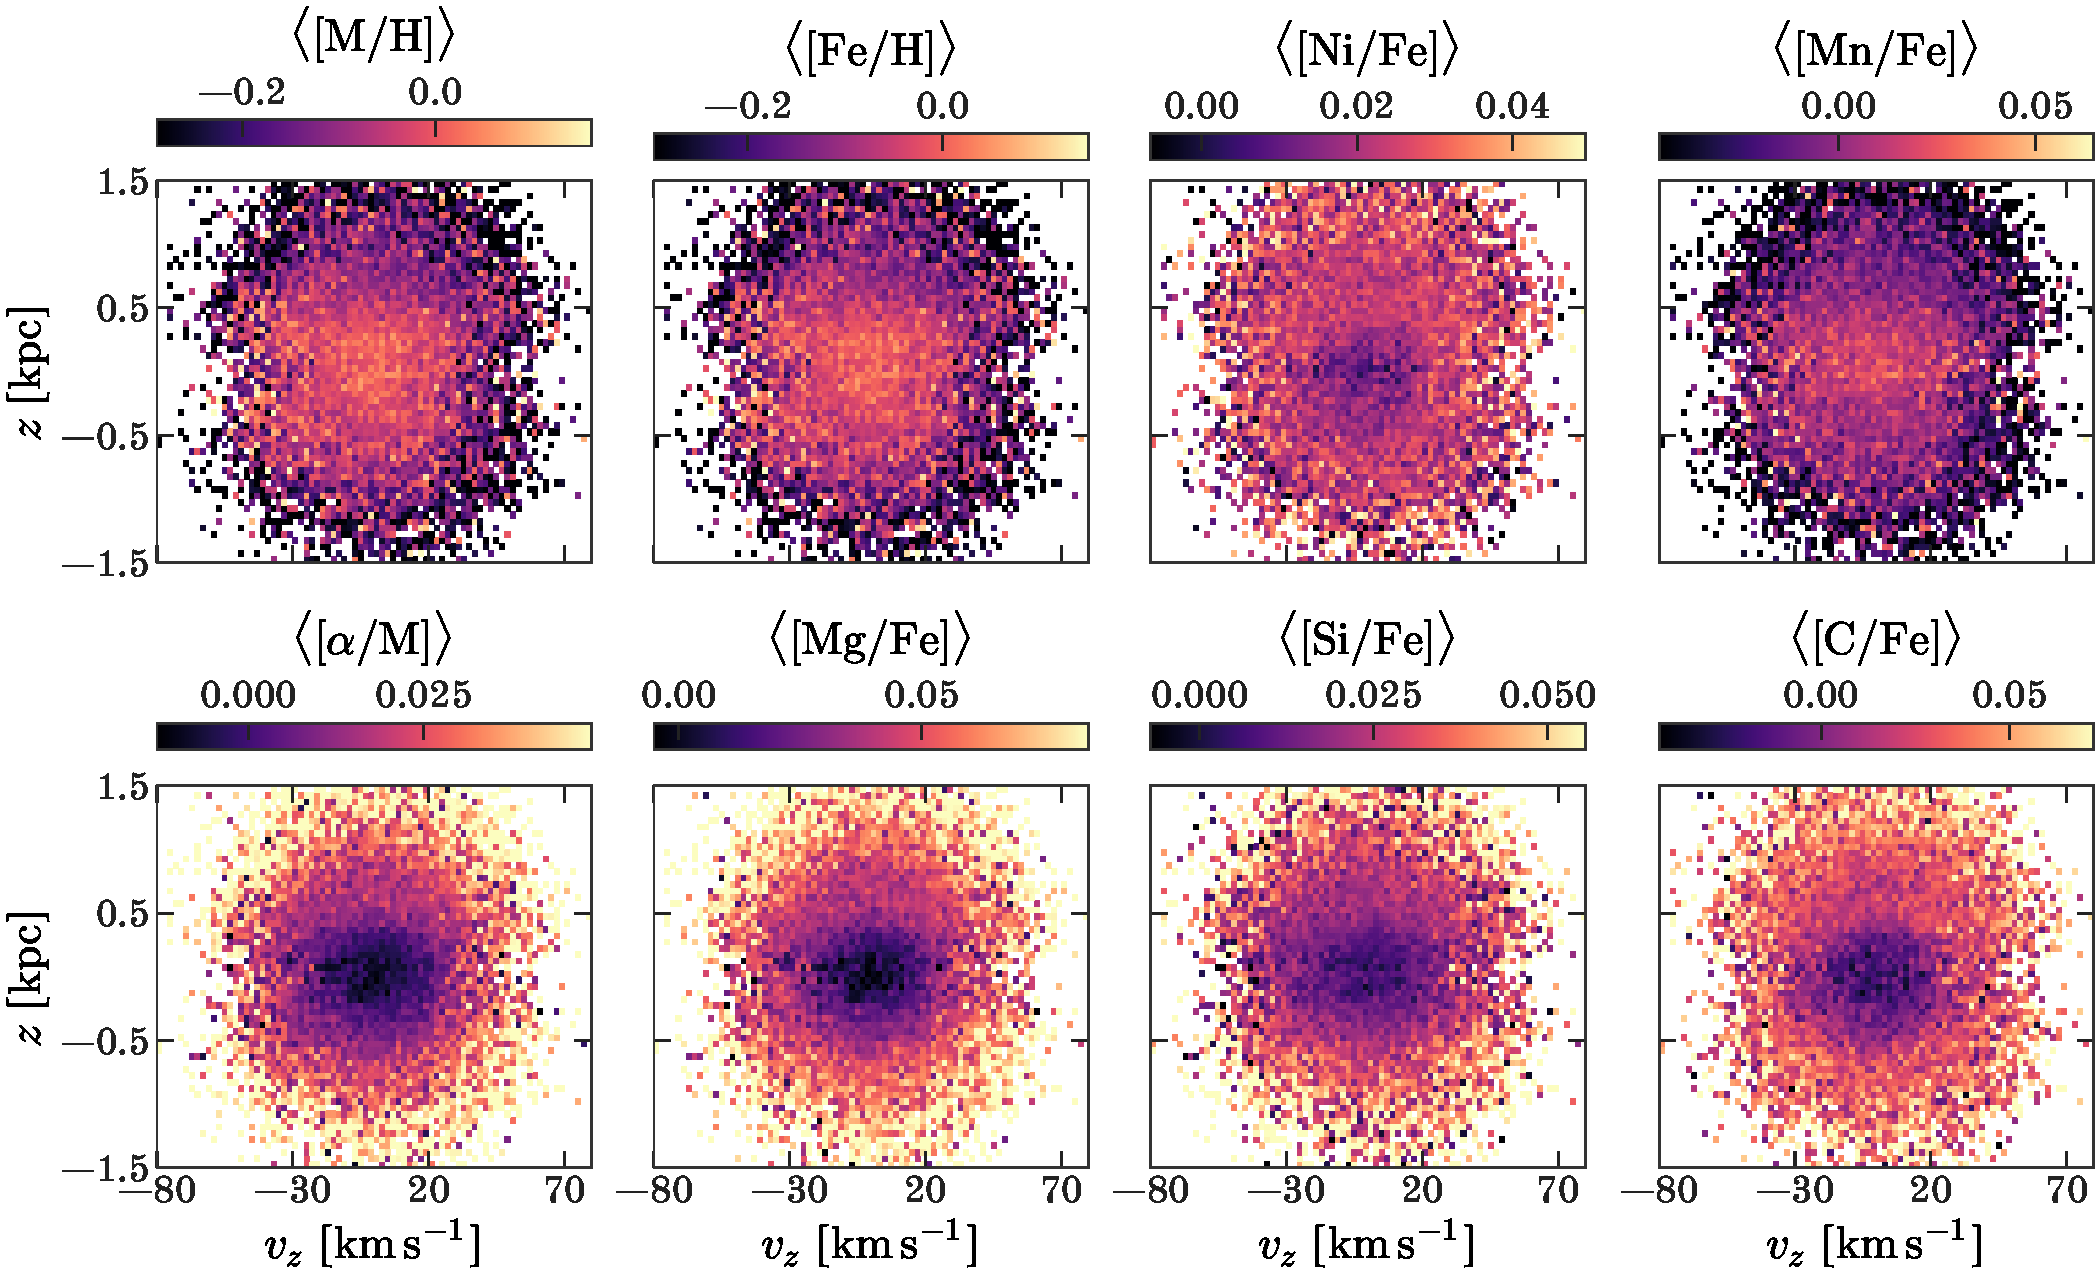
\includegraphics[width=\textwidth]{abundance-zvz-grid.pdf}
  \end{center}
  \caption{%
    The means of various (logarithmic) abundance ratios as a function of
    Galactic vertical height $z$ and vertical velocity $v_z$.
    Averages are taken in $z, v_z$ boxels.
    The stars at lower $|z|$ and lower $|v_z|$ (that is, the stars with
    lower overall vertical action $J_z$) show higher overall metallicity
    on average, but lower alpha-to-iron.
    These plots are somewhat affected by \apogee\ selection effects, in
    that different $z, v_z$ boxels are projections through different extents
    in Galactocentric radius (see \figurename~\ref{fig:mh-am-xy}).
    This explains some of the visible asymmetries.
  \label{fig:zvz-grid}
  }
\end{figure}

A significant motivation for his work came from plots of elemental abundance
ratios of stars as a function of vertical height $z$ and vertical velocity $v_z$
in Galactocentric Cartesian coordinates.
Examples are shown in \figurename~\ref{fig:zvz-grid}, which show the mean
abundance ratios of stars in bins of their vertical phase-space coordinates,
using data from the \apogee\ and \gaia\ surveys (see
\sectionname~\ref{sec:data}).
In these plots, the eye is drawn to \emph{abundance gradients}:
The stars at small heights and small vertical velocities have different
abundance ratios, on average, than stars at large heights and large vertical
velocities.
But these positional and velocity gradients are related:
Stars at large absolute vertical velocities $v_z$ will, as they orbit, reach
large absolute vertical positions $z$ (far from the Galactic plane, that is),
and stars at large absolute vertical positions will, in the future, reach large
absolute vertical velocities.
That is, the stars will orbit in the Galaxy, which projects onto this $z$--$v_z$
plane as (to zeroth order) roughly elliptical trajectories.
For example, \figurename~\ref{fig:zvz-demo} shows two Galactic orbits computed
in a 3D model for the Milky Way (see \sectionname~\ref{sec:mw-model}) in
different projections of phase-space coordinates:
In the space of $z$--$v_z$ (center panel), a Galactic orbit will form a
close-to-elliptical band whose enclosed area scales with the vertical action,
$J_z$, whose thickness depends on the eccentricity of the orbit, and a given
position on its ``ellipse'' can nearly be mapped to a vertical angle,
$\theta_z$.

% Notebook: figures/zvz-orbit-demo.ipynb
\begin{figure}[!tp]
  \begin{center}
  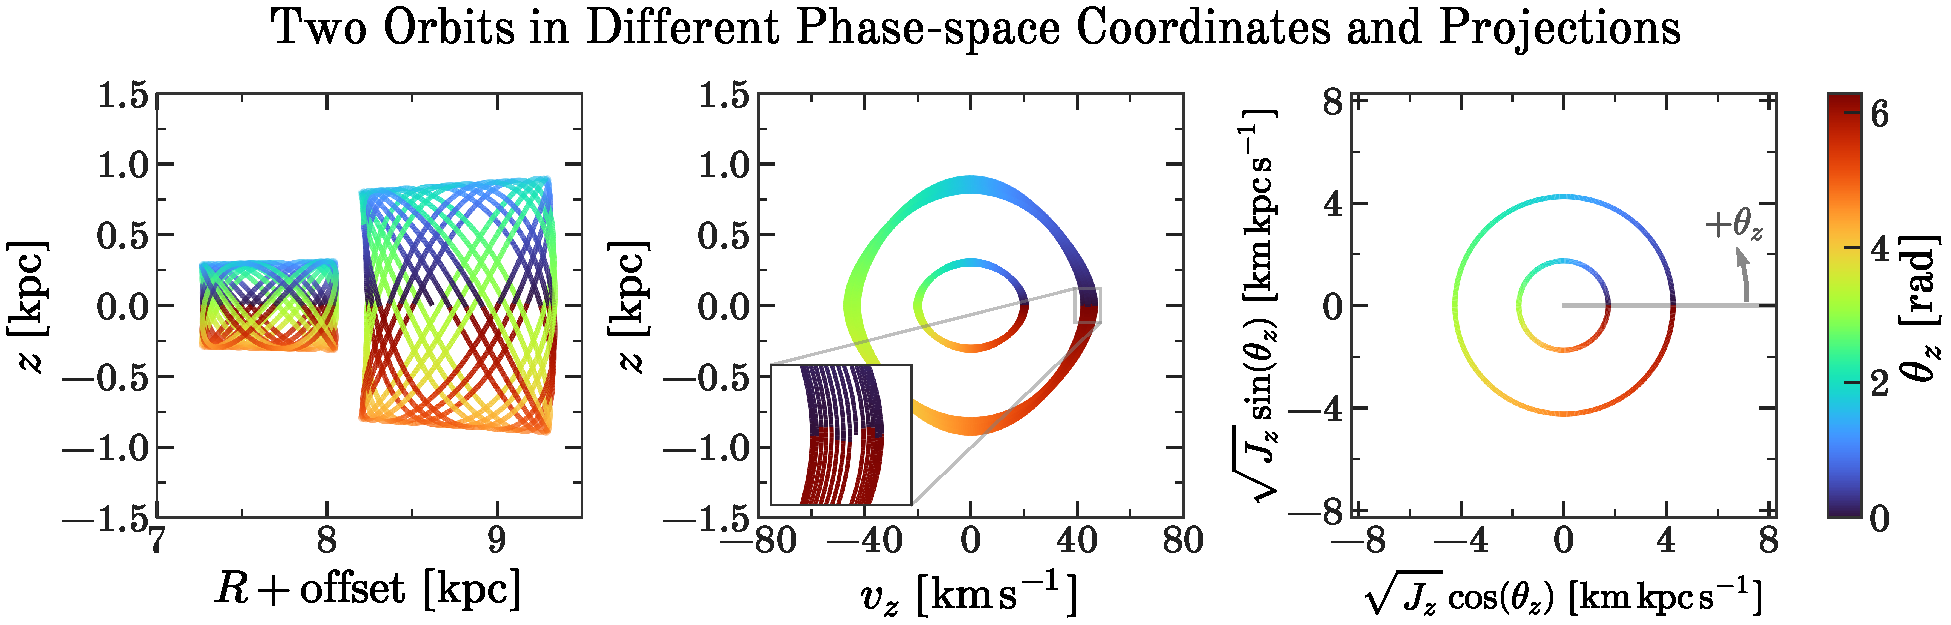
\includegraphics[width=\textwidth]{zvz-orbit-demo.pdf}
  \end{center}
  \caption{%
    \textsl{Left panel:} Two orbits projected onto the plane of
    Galactic vertical height $z$ and Galactocentric cylindrical radius
    $R$. The orbits fill the surfaces of 3-tori in 6-d phase space.
    \textsl{Middle panel:} The same two orbits, but projected onto the plane
    of vertical height $z$ and vertical velocity $v_z$. In this projection,
    it becomes clearer that the orbital lines are
    colored by the angle $\theta_z$ that is conjugate to vertical action $J_z$.
    The inset shows that conjugate angle wraps non-trivially, because the action
    (by construction) wraps at constant angular velocity, whereas the vertical period
    is a (weak) function of the other orbital phases.
    Note that although this projection is close to ``face on'' for these two
    orbits, the fact that they fills the surfaces of 3-tori means that they
    project to finite-width bands in $z, v_z$ space.
    \textsl{Right panel:} The same two orbits, but now plotted in vertical-action,
    vertical-angle space. In this space, the two orbits trace perfect circles.
  \label{fig:zvz-demo}
  }
\end{figure}

To very high precision, stars do not change their abundances as they orbit.
One consequence of this is a new method for inferring the orbit structure of the
Milky Way:
If two small neighborhoods in phase space lie on the same orbit---that is, they
correspond to the same dynamical actions but with different conjugate
angles---they must contain stars with the same distribution of element
abundances.
This prediction depends on many detailed assumptions, such as that the Galaxy is
(approximately) phase mixed, and that the potential is (approximately) time
invariant and integrable.
And of course the \emph{usefulness} of this prediction for inference depends on
the existence of gradients: If there are no element-abundance-ratio gradients,
there will be no information to exploit.

For the sake of illustration and simplicity, we visualize and demonstrate these
concepts using the vertical kinematics of stars in our parent sample.
\figurename~\ref{fig:zvz-mgfe} again shows the mean \abunratio{Mg}{Fe} abundance
ratios (in all panels), but now with two overlaid orbits (white overlaid bands)
computed in three different Milky Way models (with varied disk mass, as
indicated; see \sectionname~\ref{sec:mw-model}).
The two orbits were chosen for illustrative purposes (one with low $J_z$, one
with higher $J_z$), and are defined such that they have the same values of their
three actions $(J_R, J_\phi, J_z)$ in all mass models.
In the fiducial mass model ($\mratio = 1.0$), the two overlaid orbits nearly
follow mean abundance contours.
In the model in which the disk is made less massive (and the halo more massive
to keep the circular velocity constant; $\mratio = 0.4$), the orbits change
shape:
There is more positional extent to an orbit relative to its velocity extent.
If stars were traveling on these lower-disk-mass orbits, they would have to
obtain higher abundances when they are passing through the disk midplane,
and lower abundances when they are at their greatest absolute vertical heights,
which is absurd: Stars do not change their abundances as they orbit.
In our method below, we utilize this fact to infer the disk mass.


% Notebook: figures/APOGEE-zvz-orbits.ipynb
\begin{figure}[!tp]
  \begin{center}
  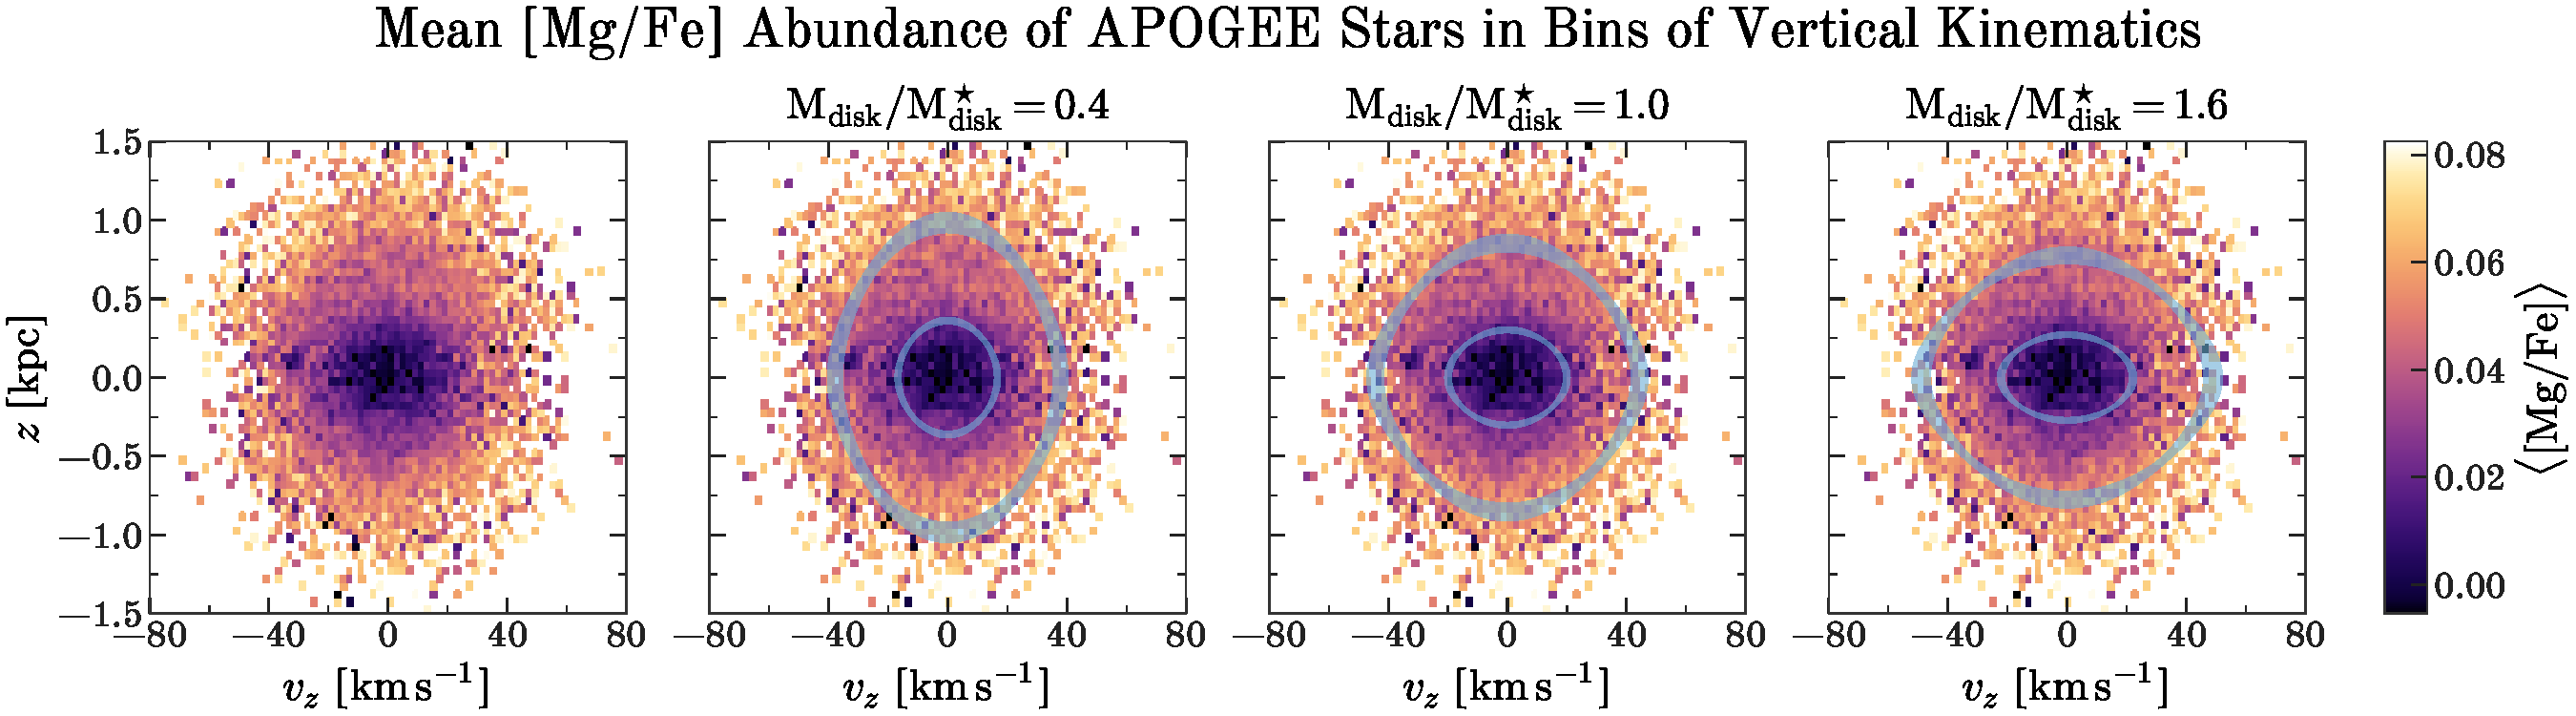
\includegraphics[width=\textwidth]{zvz-mean-MG_FE}
  \end{center}
  \caption{%
    \textsl{Left panel:} A repeat of the $\mgfe$ panel of
    \figurename~\ref{fig:zvz-grid}.
    \textsl{Other panels:} The same as the left panel, but with the two orbits
    from \figurename~\ref{fig:zvz-demo} over-plotted, for three different Milky
    Way potentials.
    These three potentials have the fiducial Milky Way disk mass (see text
    for details), or a disk less massive by a factor of 0.4 or more
    massive by a factor of 1.6, as noted in each panel title.
    All potentials are constrained to have a circular velocity at the
    Solar circle of $229\,\kms$.
    \emph{Which of the three panels appears most like the orbits are
    coincident with isopleths of the mean abundance?}
    This question is asked for illustrative purposes only: these plots distort
    the data by projection in phase space, and the methods we use for the
    inferences we perform (see \sectionname~\ref{sec:inferences})does not rely
    on projections.
  \label{fig:zvz-mgfe}
  }
\end{figure}


\section{Method, Assumptions, and Toy Applications}
\label{sec:inferences}

There are two families of approaches to \methodname:
In the first---which we will call \emph{classical} (in the sense of classical
statistics)---we make explicit the fact that the element abundance distribution
should not depend on the conjugate angles.
The best-fit or inferred mass-model parameters are those that lead to no
residual dependence of abundances (or mean abundance ratio, or any moment of the
abundance-ratio distribution) on angles.
In the second---which we will call \emph{generative}---we would construct a
predictive model for the high-dimensional abundance distribution as a function
of actions alone (and not angles).
The best-fit or inferred mass-model parameters are those that maximize the
combined probability (density), evaluated at the observed abundances.
The classical approaches are frequentist and the generative approaches produce
likelihoods and can be used in Bayesian inferences.

Both classical and generative implementations of \methodname\ depend on a
specific set of assumptions, enumerated below.
We emphasize that these assumptions are not necessarily correct, but that our
method is conditionally correct, conditioning on these core assumptions:
\begin{description}
\item[integrable] Each stellar orbit is regular and has three
  dynamically-invariant actions and three conjugate angles. This assumption
  could in principle be relaxed in future implementations.
\item[well mixed] The stars in our sample are inherently uniformly distributed
  in angle variables; all angles are equally likely. This assumption will be
  violated substantially in the data (as we discuss below; see
  \sectionname~\ref{sec:discussion}), but this is the fundamental assumption of
  the vast majority of inferences of the Milky Way mass distribution.
  % TODO: make sure to mention the Snail in the discussion
\item[selection] The selection function depends on position (or velocity) in the
  Milky Way, but not on element abundances. In detail, the \apogee\ selection
  function \emph{will} depend on abundances through gradients between stellar
  parameters and element abundance and implicit selections on stellar
  parameters. We attempt to mitigate these issues here by selecting only red
  giant stars near the red clump (see \sectionname~\ref{sec:data}), and we
  discuss this further in \sectionname~\ref{sec:discussion}.
  % TODO: Alternatively, we could use a strongly-constrained model for the
  % dependence of the selection function on element abundances.
\item[smooth gradients] \HOGGTODO{Assumption about how the abundances can
  depend on action.} Relatedly, the use of action and not log-action
  or zmax or whatever.
\end{description}

In this \documentname, we consider only classical approaches for illustrative
purposes.\footnote{This may surprise some of our readers, but we are pragmatic
as much as dogmatic about Bayes!}
The classical approaches are simpler in implementation, make fewer assumptions,
and more explicitly embody the orbits-as-isopleths concept that underlies the
project descriptions we have given above.
However, we expect that generative approaches will produce at least slightly
more precise inferences, since they will be protected by the arguments and
proofs of Bayesian inference.
In addition to the core assumptions listed above, we also make additional
assumptions specific to our implementation and demonstrations here:
\begin{description}
\item[kinematic measurements] The 6D phase-space positions are sufficiently
  accurate and precise such that we condition (or bin) over these quantities.
  For the parent sample used here, the median distance uncertainty is $\sigma_d
  \approx 50~\pc$ and the median velocity uncertainty is $\approx 2~\kms$.
\item[abundance measurements] \HOGGTODO{Assumption that stars in different parts
  of phase space get the same abundance measurements.} Questionable in certain
  kinds of samples.
\end{description}

For simplicity, we focus here on the vertical kinematics of stars and we ask
whether there is a choice of mass model that leads to dynamical actions and
conjugate angles such that the abundance ratio distributions do not depend on
the conjugate angle $\theta_z$.
We fix all aspects of our mass model except for the ratio of the disk mass to
the halo mass at fixed circular velocity (see \sectionname~\ref{sec:mw-model}).
To assess the dependence of a particular element abundance ratio
\abunratio{X}{Y} on the vertical angle, we define a ``mean abundance-ratio
deviation,'' $\Delta^{\abunratio{X}{Y}}$, for each $n$ star, which is the
difference between a given star's (logarithmic) abundance ratio and the mean of
the (logarithmic) abundance ratios of its kinematic neighbors (in action-space),
\begin{equation}
  \Delta^{\abunratio{X}{Y}}_n = \abunratio{X}{Y}_n -
    \left\langle \abunratio{X}{Y} \right\rangle_{\vec{J}}
    \quad .
\end{equation}
That is, we use a given mass model to compute the three actions $\vec{J}$ for
each star in the parent sample and choose the closest $K$ neighbors in
$\vec{J}$-space (with the isotropic Euclidean metric distance) for each star to
compute the action-local mean abundance.
For a specific star, its neighbors are a function of the mass-model parameters
because all actions will change values in different mass models.
We choose to use $K=64$ based on experimentation, but find that our results are
insensitive to this choice.
\todo{Actually, we do a crazy weighted mean!}

Our goal then is to minimize (over mass model parameters) the dependence of the
mean abundance-ratio deviation distribution on the vertical angle $\theta_z$.
To quantify this dependence, we fit a smooth model of the form
\begin{equation}
  \Delta(\theta_z) = c_0 + a_1\,\cos  \theta_z + b_1\,\sin    \theta_z
                         + a_2\,\cos 2\theta_z + b_2\,\sin 2\theta_z \quad,
                         \label{eq:fouriermodel}
\end{equation}
where the five parameters $(c_0, a_1, a_2, b_1, b_2)$ are the coefficients of a
Fourier series expressed out to $m=2$.
We fit this model to all of the $N=\nstars$ individual abundance-ratio
deviations and their uncertainties $(\Delta_n, \sigma_{\Delta_n})_N$ (without
binning) using least-squares fitting.
This functional form captures our expectations for how the mean abundance-ratio
deviations will depend on vertical angle when our model is wrong:
If the orbit contours at a given action have the wrong shape, we expect there to
be an $m=2$ variation to the abundance-ratio deviations (e.g.,
\figurename~\ref{fig:zvz-mgfe}).
If our assumed solar position relative to the midplane or solar velocity
relative to the local standard of rest are wrong, we expect there to be $\sin$
and $\cos$ (i.e., $m=1$) variations.

\figurename~\ref{fig:sinusoid-fits} shows smooth fits of the above model
computed from bootstrapped resamplings of the data (blue curves) and, for
visualization only, we show binned means of the measured abundance-ratio
deviations (black histogram).
We emphasize that no binning is performed at any time in performing these fits.
The results shown in \figurename~\ref{fig:sinusoid-fits} are for abundance
deviations in $\mgfe$, and just for three particular settings of the disk mass
parameters, \mratio.
The data are bootstrapped prior to the construction of the abundance deviations,
because the abundance-deviation estimates depend on the data set in play, and
also the mass-model parameters.

\begin{figure}[!tp] % Notebook: figures/Abundance-anomaly-bootstrap.ipynb
  \begin{center}
  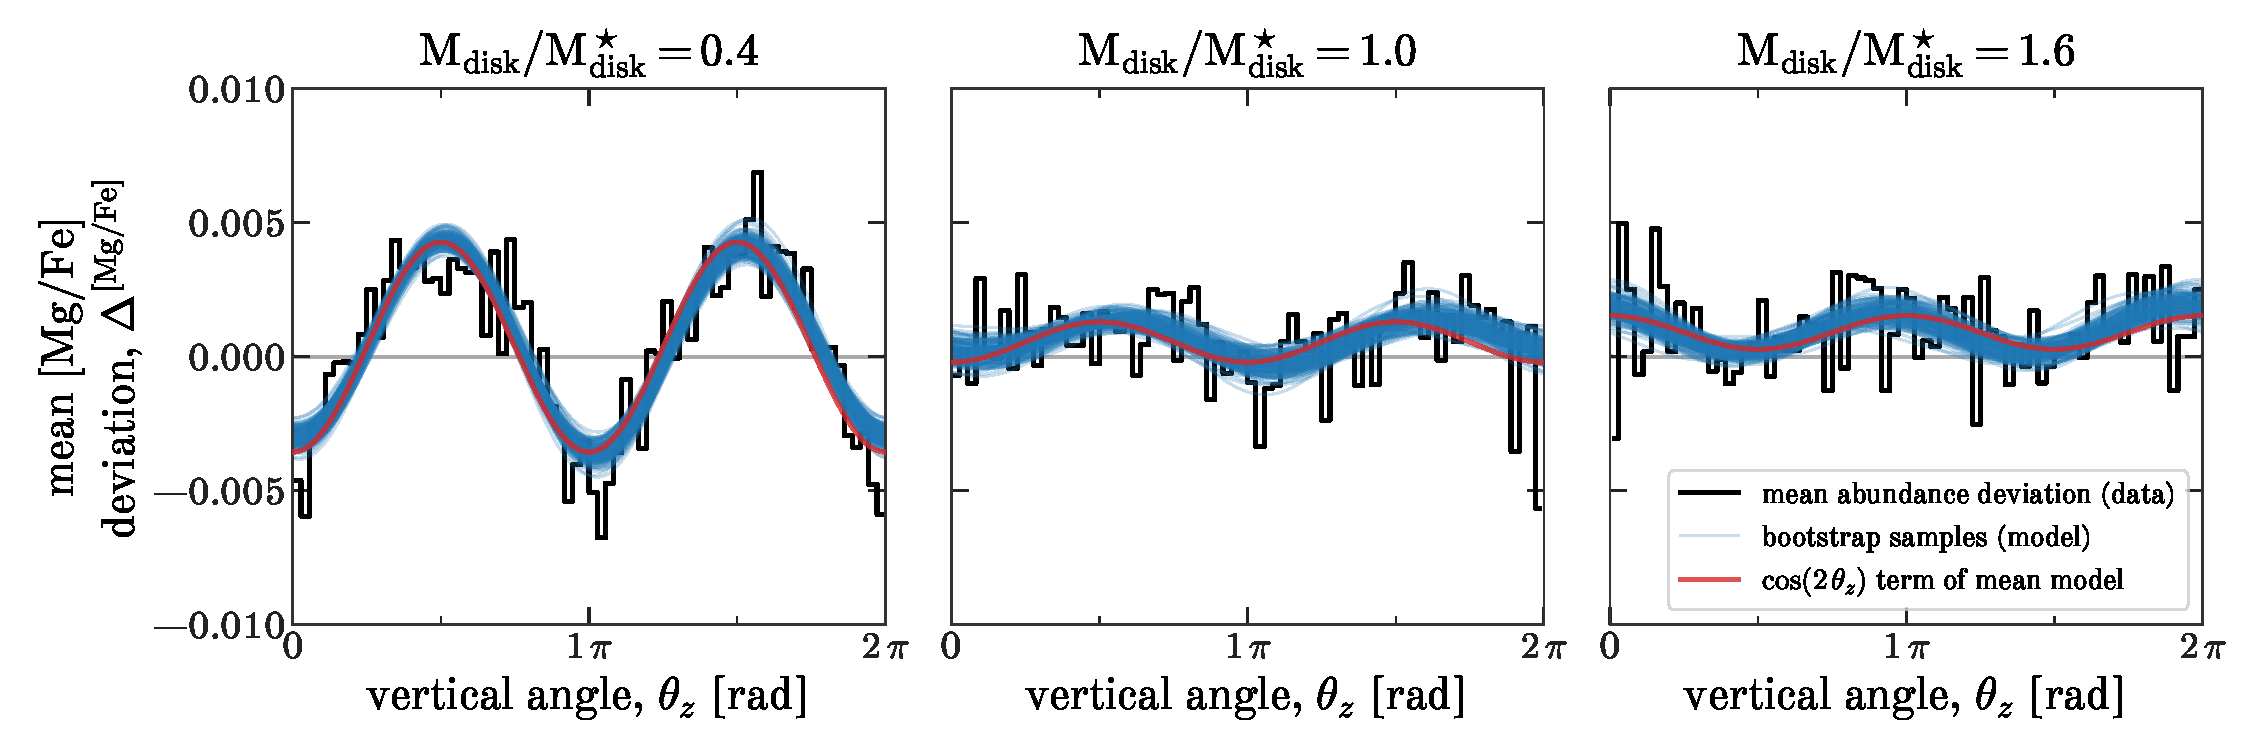
\includegraphics[width=\textwidth]{sinusoid-fits.pdf}
  \end{center}
  \caption{%
    The mean $\mgfe$ abundance deviation, $\Delta^\abunratio{Mg}{Fe}$, as a
    function of vertical angle, for three different values of the mass of the
    disk (at fixed circular velocity at the Solar circle).
    The abundance deviation for each star in the sample is the difference
    between the abundance measured in each star and a mean of the $K=64$ nearest
    neighbors to that star in three- dimensional action space (for that mass
    model).
    In each panel, the mean abundance deviation is shown three ways.
    The black histogram shows the mean of the abundance deviation in small bins
    in vertical angle.
    The blue lines show continuous fits to the unbinned data, which are
    continuous linear combinations of sines and cosines (see
    \sectionname~\ref{sec:inferences}); there are 128 blue lines, one for each
    of 128 independent bootstrap trials.
    The red line shows the mean of the $\cos 2\,\theta_z$ terms across the
    128 bootstrap trials.
    Although the black line shows binned means for visualization purposes,
    these bins are never used in the analysis (binning is sinning and all that).
    Comparing the three panels, the red curves show an amplitude of opposite
    sign in the highest-disk-mass panel relative to the other panels, suggesting
    that the best setting of the disk mass is in between the fiducial disk mass
    model and the higher-disk-mass model (as we find; see
    \sectionname~\ref{sec:inferences}).
  \label{fig:sinusoid-fits}
  }
\end{figure}

In the smooth model for the mean abundance deviations
(\equationname~\ref{eq:fouriermodel}), the parameter $a_1$ is sensitive to the
vertical component ($v_z$ component) of the local standard of rest or the Solar
motion.
Parameter $b_1$ is sensitive to the vertical ($z$) location of the Sun relative
to the disk midplane.
Parameter $a_2$ is sensitive to the local mass density concentrated in the disk,
or the disk-mass parameter \mratio.
Parameter $b_2$ should not exist and is included as a test of model assumptions;
in detail, it is sensitive to tilts in the coordinate system, and
non-phase-mixed structures.
Note that the sign of the $m=2$ term flips between the left and right panels of
\figurename~\ref{fig:sinusoid-fits}, indicating that the ``best-fit'' mass model
must be at an intermediate value of $\mratio$, close to but slightly larger than
the fiducial value.

We repeat this fitting procedure for a grid of disk mass parameter values
$\mratio = 0.4$--$1.8$:
For each mass model (i.e., each setting of \mratio), we estimate the Fourier
coefficient parameters and uncertainties on the coefficients using 128 bootstrap
trials.
\figurename~\ref{fig:coeff-mdisk} shows the inferred coefficients for the
abundance ratio \mgfe\ as a function of disk mass \mratio.
Conceptually, to turn this into a constraint on the disk mass, we then look for
the value of \mratio\ that minimizes the (absolute) value of $a_2$.
We obtain an estimate for the disk mass parameter \mratio\ and an associated
uncertainty by linearly interpolating the measurements and bootstrap error bars
onto the $a_2=0$ intercept.
Our ``best-fit'' disk mass and its uncertainty is shown as the square (blue)
marker in \figurename~\ref{fig:coeff-mdisk} to emphasize that, though this is a
simple model and we only vary one parameter in this demonstration, the
measurement is encouragingly precise with a formal error bar of $\approx$7\% for
just a single element abundance.
% This value, and its uncertainty, are shown in the lower-left panel of
% \figurename~\ref{fig:coeff-mdisk} as the square marker with a horizontal
% error-bar.
We note that here we also apparently measure a finite value for the $\sin
2\theta_z$ term, which should not exist in the universe defined by our
assumptions (and is therefore labeled ``verboten'').
This implies that our assumptions seem to be lightly violated (the inferred
amplitude is only marginally significant), and we discuss this further in the
context of our assumptions below (\sectionname~\ref{sec:discussion}).


\begin{figure}[!tp] % Notebook: figures/Abundance-anomaly-bootstrap.ipynb
  \begin{center}
  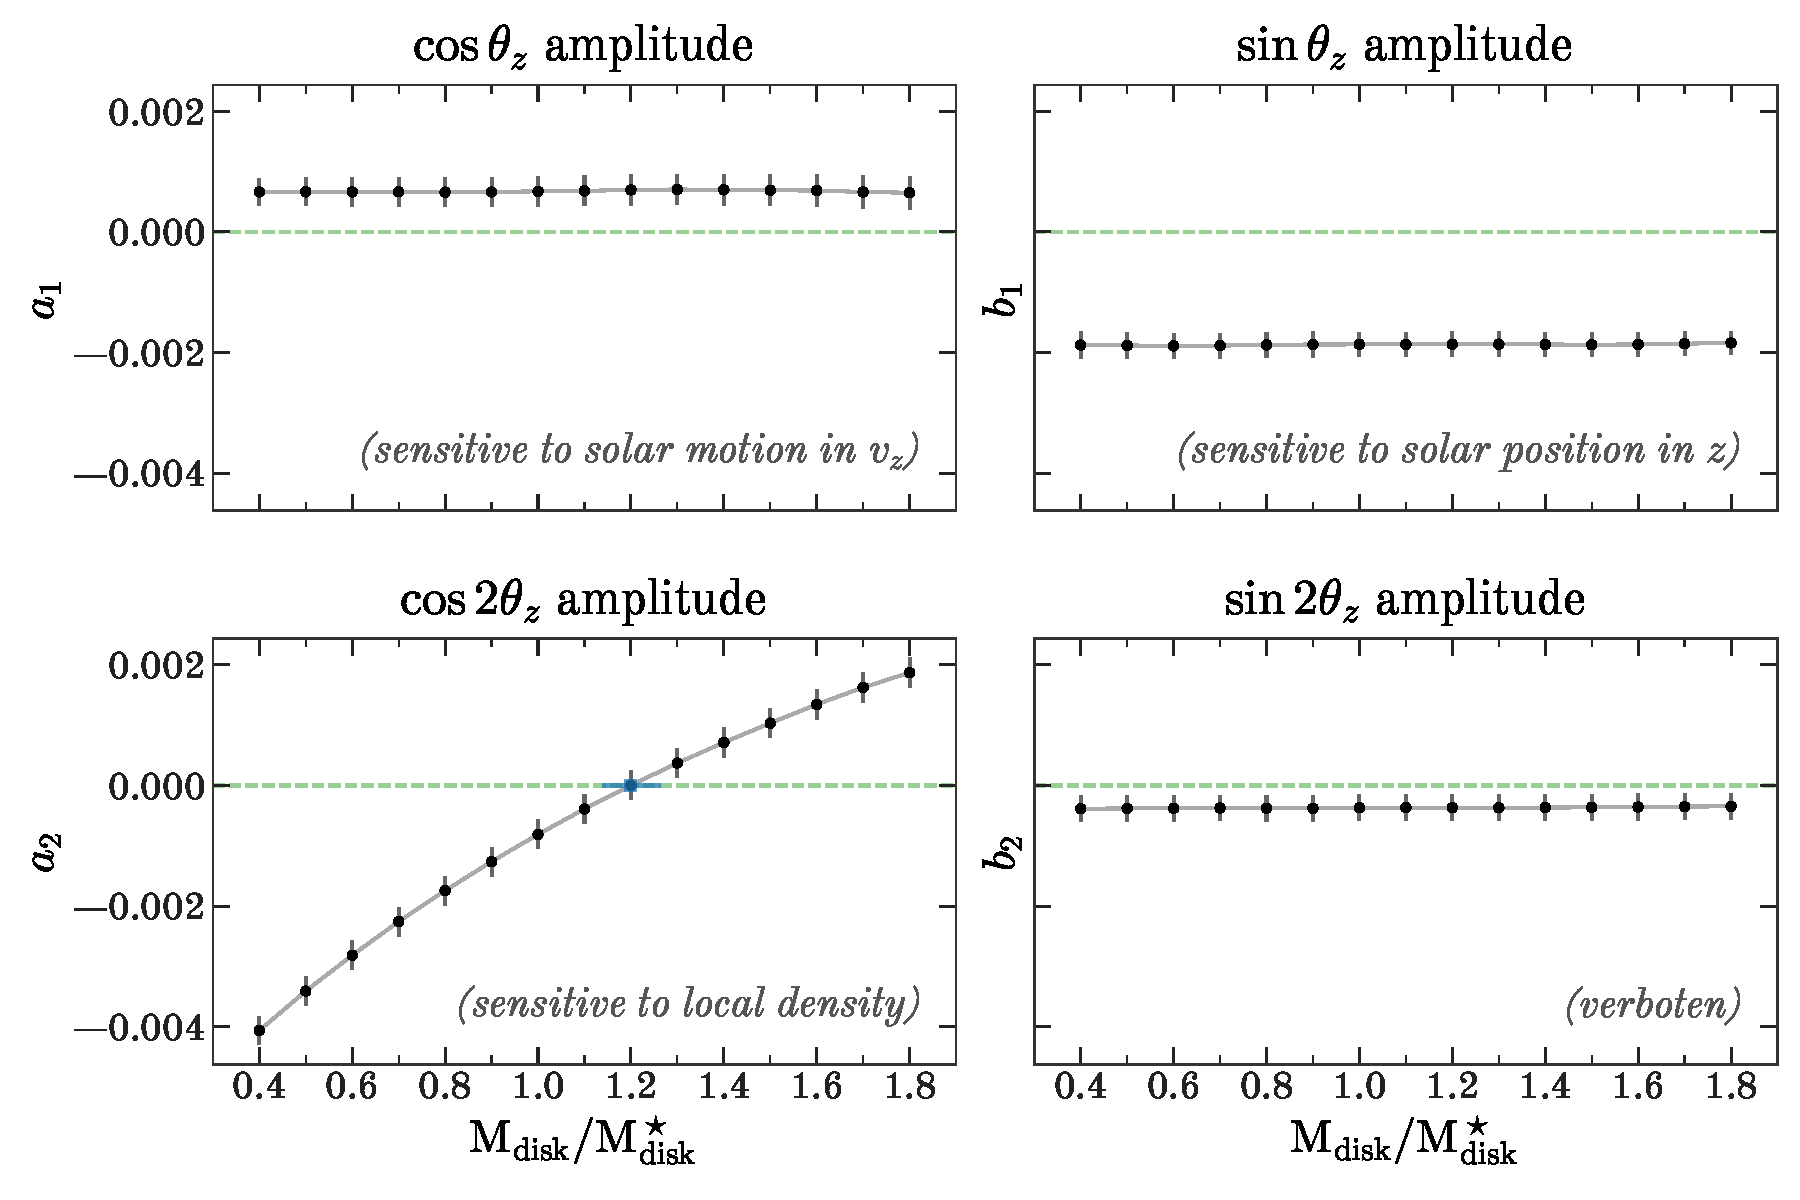
\includegraphics[width=0.9\textwidth]{coeff-vs-mdisk.pdf}
  \end{center}
  \caption{%
    Parameters of the smooth sine-and-cosine fits to the dependence of \mgfe\
    abundance deviation on vertical angle $\theta_z$ (the blue lines in
    \figurename~\ref{fig:sinusoid-fits}), as a function of the disk-mass
    parameter \mratio.
    The black markers show the values of the disk-mass parameter at which we
    performed the sine-and-cosine fits; the vertical error bars show the
    bootstrap uncertainties for each coefficient.
    The amplitude of the $\cos 2\theta_z$ term is the amplitude that is
    sensitive to the local density of the disk; it crosses zero when the model
    has the best-fit disk mass.
    The best-fit disk mass and its measurement uncertainty are shown as the
    square marker and a horizontal error bar.
    The other terms shown have different dependencies on Milky Way parameters:
    The $\cos\theta_z$ would vary strongly if we varied the solar motion (the
    vertical component of the local standard of rest).
    The $\sin\theta_z$ term would vary strongly if we varied the location of the
    midplane of the disk.
    The $\sin 2\theta_z$ term cannot be non-zero; the fact that we find a
    non-zero value for this amplitude may suggest a weak violation of our model
    assumptions (see \sectionname~\ref{sec:inferences}).
    These figures show that we can precisely measure the disk mass.
  \label{fig:coeff-mdisk}
  }
\end{figure}

% Another thing we can glean from \figurename~\ref{fig:coeff-mdisk} is that these
% data seem to favor a different value of the solar position relative to the
% midplane $z_\odot$ and a different solar velocity $v_{z, \odot}$.
The upper panels of \figurename~\ref{fig:coeff-mdisk} show that, at all values
of the disk mass parameter \mratio, there is a finite $m=1$ amplitude for both
the $\cos$ and $\sin$ terms.
As noted before, these coefficients are sensitive to the solar motion and solar
position (in $z$), respectively.
We therefore simultaneously optimize over the disk mass parameter \mratio, the
solar position relative to the midplane $z_\odot$, and the solar $z$ velocity
relative to the local standard of rest $v_{z, \odot}$.
For each value of our parameters $mratio, z_\odot, v_{z, \odot}$, we compute the
Fourier coefficients and minimize the objective function
\begin{equation}
  f(a_1, b_1, a_2 \,;\, \mratio, z_\odot, v_{z, \odot}) =
    a_1^2 + b_1^2 + a_2^2 \quad . \label{eq:objective}
\end{equation}
Note that here we ignore the constant term $c_0$ and the amplitude of the $\sin
2\theta_z$ term $b_2$.
We again perform 128 bootstrap trials per element, and we perform the bootstrap
resampling outside of the entire procedure (so that each optimization is
performed independently with a bootstrap sample).
We use Nelder-Mead optimization \citep{Gao:2012} to minimize our objective
function, as implemented in the \package{scipy} package \citep{scipy}.

\figurename~\ref{fig:elem-ellipses-1} shows a summary of our constraints on the
disk mass parameter and solar velocity for all of the elements shown in
\figurename~\ref{fig:zvz-grid} (colorful ellipses), and the joint constraint
from all of these elements combined (dark, black ellipse).
Here we show one- and two-sigma error ellipses (darker and lighter ellipses for
each color), with means and covariance matrices estimated from the optimization
results for the bootstrap resamplings of the data for each abundance ratio.

% \begin{table}[ht]
%   \footnotesize
%   \centering
%   \begin{tabular}{c | c}
%       % \multicolumn{3}{c}{\textbf{Summary of Results}} \\
%       \hline
%       Parameter & Inferred Value\\
%       \hline
%       ${\rm M}_{\rm disk}$ (total) & $7.88 \pm 0.19 \times 10^{10}~\Msun$ \\
%       ${\rm M}_{\rm disk} / {\rm M}_{\rm halo} (<8.1~\kpc)$  & $2.06 \pm 0.05$\\
%       $z_{\odot}$ & $15.5 \pm 1.0~\pc$\\
%       $v_{z, \odot}$ & $8.6 \pm 0.2~\kms$\\
%       \hline
%   \end{tabular}
%   \caption{For your consideration: Some numbers that have no relevance.
%   }
%   \label{tbl:results}
% \end{table}

% We have shown results for the $\mgfe$ abundance deviation, but we repeat this
% analysis for several different abundances (the same abundances as shown in
% \figurename~\ref{fig:zvz-grid}).
% The full set of disk-mass measurements are shown in
% \figurename~\ref{fig:inferred-mdisk-elems}.
% The different abundances tell somewhat different stories, but the combined total
% precision of this measurement is very high, on the order of $\sim 4$ per cent in
% the mass of the Milky Way disk, locally.

% % Notebook: figures/Abundance-anomaly-bootstrap.ipynb
% \begin{figure}[!tp]
%   \begin{center}
%   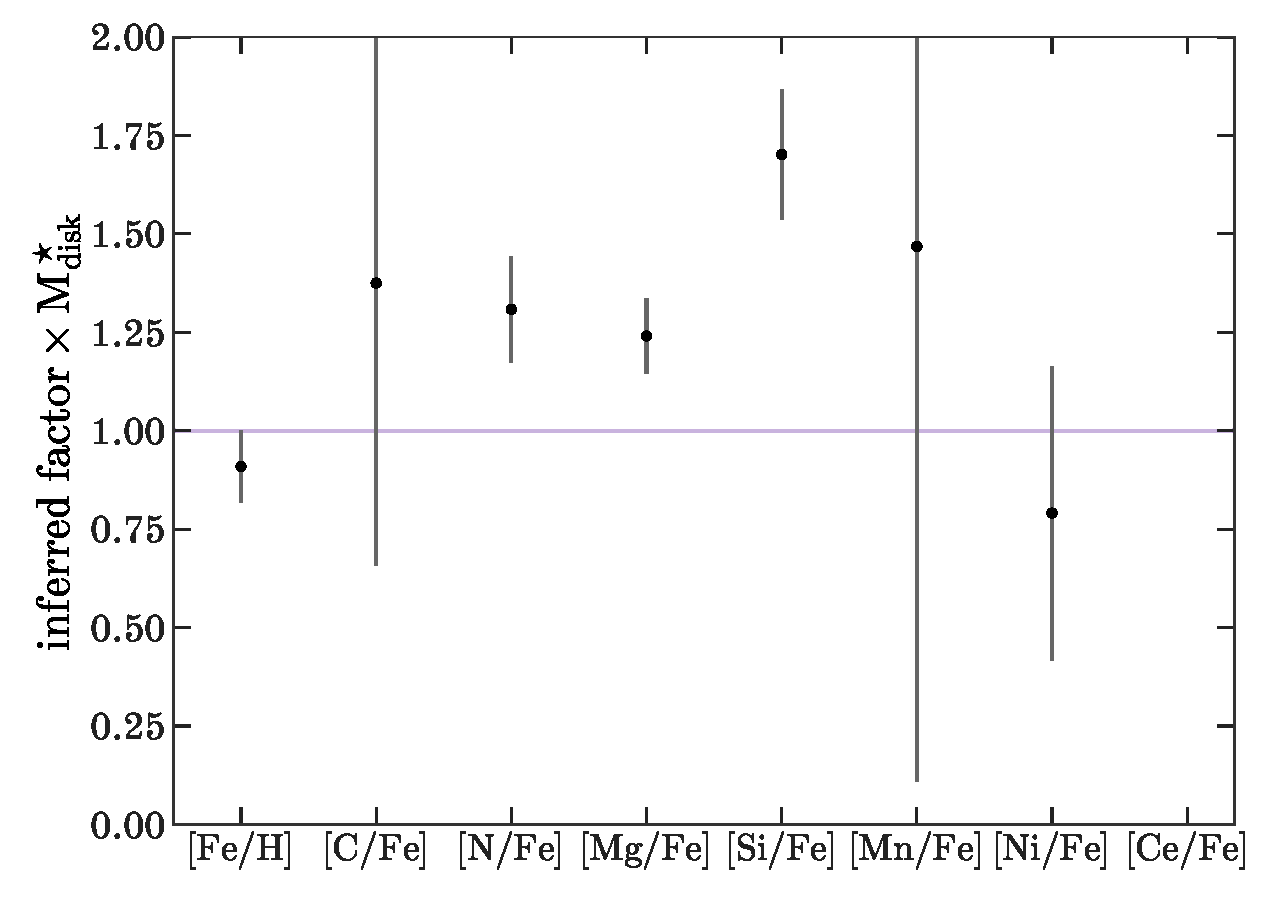
\includegraphics[width=\textwidth]{mdisk-vs-elem.pdf}
%   \end{center}
%   \caption{%
%     Our measurements of the disk mass from each of several abundance ratios.
%     The measurement shown in the $\cos 2\theta_z$ (lower-left) panel of
%     \figurename~\ref{fig:coeff-mdisk} is shown here as the $\mgfe$ measurement.
%     The horizontal (purple) band shows the inverse-variance-weighted mean value
%     for the disk-mass parameter $\mratio$ and its formal uncertainty.
%     This figure shows that the different element abundance ratios deliver
%     somewhat inconsistent estimates for the disk mass; these inconsistencies are
%     discussed in the text.
%   \label{fig:inferred-mdisk-elems}
%   }
% \end{figure}

% Notebook: figures/5-Optimize-results.ipynb
\begin{figure}[!tp]
  \begin{center}
  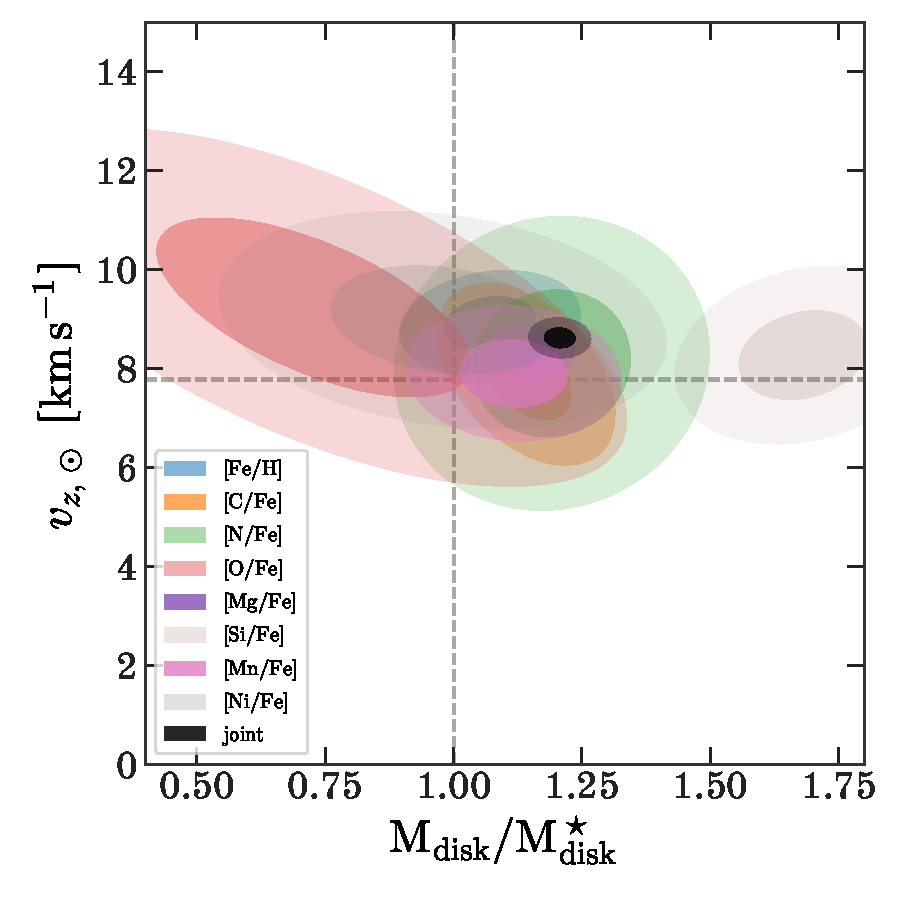
\includegraphics[width=0.6\textwidth]{M-vz-error-ellipses.pdf}
  \end{center}
  \caption{%
    TODO
  \label{fig:elem-ellipses-1}
  }
\end{figure}

% Notebook: figures/5-Optimize-results.ipynb
\begin{figure}[!tp]
  \begin{center}
  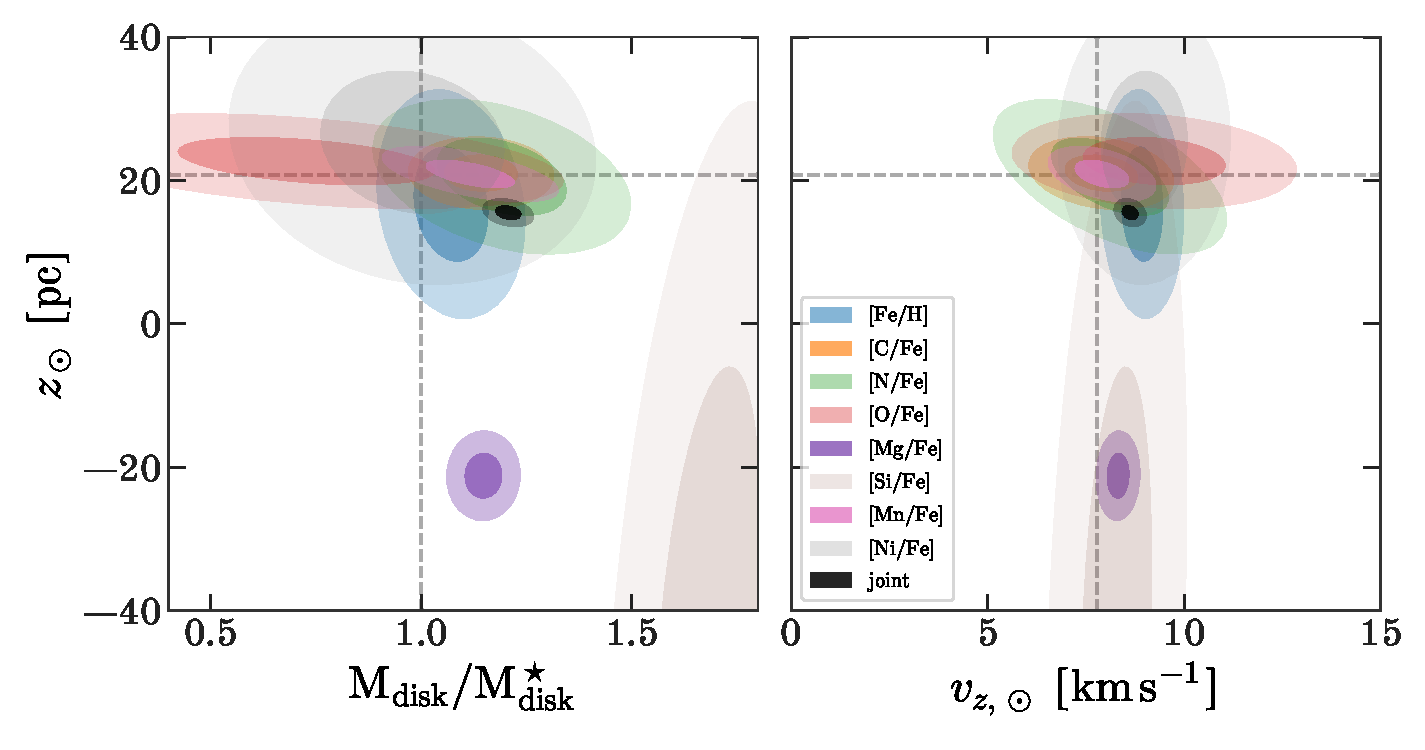
\includegraphics[width=0.8\textwidth]{M-z-vz-z-error-ellipses.pdf}
  \end{center}
  \caption{%
    TODO
  \label{fig:elem-ellipses2}
  }
\end{figure}


\section{Discussion}
\label{sec:discussion}

\subsection{What have we created?}

In this \documentname, we have presented a novel method---\methodname---for inferring
the mass model (or force law or gravitational potential) of an
integrable, angle-mixed stellar distribution.
This method does not involve second moments of velocity (like the
virial theorem and the Jeans equations do), and it does not depend on
separability or any other mathematical properties other than
integrability and angle mixing.
That is, we have a method that is more statistically stable and less
restricted than Jeans modeling.
It does, however, depend on the existence of element-abundance
gradients; the stars on different orbits (with different actions) must
have---on average or statistically---different compositions.
Fortunately these gradients are ubiquitous and strong in the Milky Way
(and most galaxies; CITE).

There are many ways to describe the fundamental prediction or structure
of \methodname. Here are a few:
\begin{description}
\item[Kinematic picture]
  Stars don't change their abundances as they orbit!  Stellar
  abundance ratios can depend on the three invariant actions, but they
  can't depend on the conjugate angles, which wind up arbitrarily with time.
\item[Local geometric picture]
  Abundance gradients taken in 6-dimensional phase space will be
  locally perpendicular, everywhere, to the orbital 3-tori in phase space.
  That is, all 6-vector gradients of all possible statistics of all possible
  element-abundance ratios must be locally perpendicular to the 3-dimensional
  hyperplane locally kissing the orbital torus at that position in phase space.
  Equivalently, at every location in 6-d phase space, there full set of 6-d
  abundance-moment gradient vectors will span a
  local 3-dimensional subspace.
  This local subspace will be orthogonal to the surface of the orbital torus
  at that location.
\item[Global geometric picture]
  The 6-dimensional phase space is foliated by a complete set of 3-tori,
  each of which is specified by the three actions.
  The orbital tori will be level 3-surfaces (in the 6-dimensional phase space) of any
  moments or statistics of the element-abundance distribution.
\item[Information-theory picture]
  Any predictive model for the element abundances of stars
  that is given the freedom to depend on both actions and angles will do no
  better at predicting stellar element abundances than a model that is only
  given the freedom to depend on actions alone.
  That is, in the 6-dimensional phase space, only the action coordinates provide
  information about the element abundances.
\end{description}

Because \methodname\ depends on measuring changes in moments of the
abundance-ratio distribution (means, in this \documentname), we
conjecture that the precision with which the mass model can be
constrained increases (the uncertainties decrease) as the
abundance-moment gradients get stronger.
By the same token, the precision will increase as the width or
dispersion of the local (in phase space) abundance distribution gets
smaller.
This dispersion will have contributions from the true distribution of
abundances and also observational uncertainties.
And of course the precision will increase as the number of stars increases,
and their coverage of the conjugate angles increases.

In this \documentname, we focused on means of (logarithmic) abundance
ratios.
But we are not restricted to these element-abundance moments; any moments
are fair game. The method also does not assume that the element abundances
are uniquely or even relatively specifically predicted by the actions:
The method only requires that there be some gradients in some moments of
the abundance distribution. There can be---and there is---a wide range of
abundance ratios at every point in action space.
In this project, all distributions are expected to have (and are observed
to have) substantial dispersion.

\subsection{How is this better than everything before?}

We assert that \methodname\ is unlike Jeans modeling, and (in
particular) that it is more stable and less mathematically constrained.
The stability claim flows from the observation that, given a sample of
stars, it is harder to precisely measure second moments than first
moments.
Any method that requires measurements of spatial derivatives of second
moments will be limited in precision.
The mathematical constraint claim flows from the point that most Jeans
models involve assumptions of separability that do not enter here.
We require gradients, but not separability.
We choose in this \documentname\ to focus on vertical kinematics, but
we nowhere assume that these vertical kinematics are separated from the
radial kinematics.
Indeed the orbits plotted in \figurename~XXXX
show finite-width projections onto the vertical phase space because we
have not performed any kind of separation or separability approximation.

Another advantage over Jeans modeling is that
we do not require knowledge of the survey selection
function, provided that the selection is made in position space (or phase
space) and does not act at all in the element-abundance ratios that
enter into the inference.
This condition is satisfied for the \apogee\ data used here, and will be for
most other surveys like it.

In some ways, \methodname\ is related to the concept of ``extended
distribution functions'' (CITE and CITE), in which the dynamical
distribution function in action space $p(\vec{J})$ is extended into a distribution
function in actions $\vec{J}$, abundances $\vec{X}$, and (perhaps)
other (near-) invariants to make a larger distribution function $p(\vec{J},\vec{X})$.
So far, extended distribution functions have not been used as tools
for inferring the mass model for the Galaxy. But they could be, in principle.
The most natural projects in this direction would require knowledge of the
selection function, however, and would therefore be harder to implement in
current surveys.

\methodname\ is also closely related to the concept of ``mono-abundance
populations'' (CITE and CITE), which have been used to look at the structure
of the galaxy, divided by element abundances.
These projects can be seen as factorizing out of the extended distribution
function $p(\vec{J},\vec{X})$ a conditional distribution
$p(\vec{J}\given\vec{X})$, although that is not precisely how they were
formulated.
In contrast, this project can be seen as factorizing out the other conditional
distribution $p(\vec{X}\given\vec{J})$, although in what's above, we don't do
so explicitly.
The great advantage of the latter factorization is that it doesn't require
knowledge of the survey selection function, provided that the selection acts
compltely in position or action space (and not ever abundance space).

One of the crazy things about a fully general statement of \methodname\ is
that any description of a general distribution in $D$-space
requires a \emph{lot of parameters}.
Even the normal distribution requires $0.5\,D\,(D+3)$ parameters for its
complete description, and anything more complex has more.
That means that there are a very large set of element-abundance statistics for which the
6-vector gradient exists or could be constraining for this project.
Not all of these parameters can be reliably measured in a finite data set,
let alone reliably seen to vary with phase-space location.
But many can.
We have discovered, in effect, a \emph{combinatorically large set of constraints on the
dynamical actions} and thus the mass model.

\subsection{What are the problems with our assumptions?}

HOGG: Return to the assumptions; do any need more discussion?

HOGG: Another is the good abundances and selection assumptions: Do the abundances affect
the selection, and are the abundance measurements a function of stellar type? Either way,
we will inherit biases.

Does the existence of a non-zero ``verboten'' term imply a violation of our
assumptions?
Or is it just bad luck?

HOGG: Finally, how sensitive are we, really, to the assumption of
phase mixing? In principle, very. But in practice: You can look at the
snail and see its aspect ratio. And that is literally a
non-phase-mixed structure. So there will be generalizations of this
method that don't depend as strongly on phase mixing. This connects,
conceptually, to work on streams in the Milky Way halo.

The flip side of that is that there are places in phase space where
mixing is maybe incredibly slow, like at low $J_z$. Maybe our disk
midplane issues come from this?

HOGG SAY: The fact that different abundances give
different disk masses, and the fact that the midplane is off, might
both be related. I think we should check whether the disk-mass results
become more consistent if we use a better disk midplane.

What is the source of our scatter in our abundance means: Shot noise
or wrongness of the assumptions?

\subsection{How can this be extended?}

... The point that there will be frequentist statistics or
optimizations, and also Bayesian approaches.  The point that Bayes and
frequentism look very different here. Call out to orbital roulette,
and to Bovy et al.

We should probably use a flexible
model for the abundance means, like a GP or etc.

That there is a fully data-driven formulation of this problem; ie, not
parameterized.

HOGG: What is the limit of this method as we go forward: Many abundance ratios? Many other
statistics of the abundance distribution? How do things change if the abundances track
each other exactly? Is that a problem? Note that we scale much better than chemical tagging
here.

HOGG: For example, we worked with the vertical angle $\theta_z$. It
would not have been a good idea to work with the azimuthal angle
$\theta_\phi$. Why not? Because the sample doesn't cover a large range
in $\theta_\phi$. But what about the angle $\theta_R$? If we had
worked with this angle we would have made an independent measurement
of the mass of the disk. We could also have used that angle to measure
the circular velocity, in the same way that the vertical angle can be
used to measure the local vertical standard of rest.

HOGG: What other tags could we have used? Other moments of other tags?
Combinations of tags? What might we gain?

Could we have used the \emph{other} actions as tags? Yes and no: Not if
their pdfs depend on selection, which they do.

...The point that this would be more complex in chaotic regions, and
maybe effectively inapplicable? Or maybe?

That this could be used to calibrate or improve abundances, in
principle!

\section{Conclusions}
\label{sec:conclusions}

Adrian, apparently, thinks that an abstract isn't enough.


\acknowledgments
It is a pleasure to thank
  Jo Bovy (Toronto),
  Anna-Christina Eilers (MIT),
  Suroor S. Gandhi (NYU),
  David Spergel (Flatiron),
  Eugene Vasiliev (Cambridge),
  the Dynamics and Astronomical Data groups at the Flatiron Institute,
  and the Galaxy group at the MPIA
for valuable discussions and input.
DWH was partially supported by HOGG GRANT DETAILS.
HWR was partially supported by GRANT DETAILS.
This research was conducted in part at the Aspen Center for Physics,
which is supported by National Science Foundation grant \acronym{PHY-1607611}.

SDSS or whatever SPECTROSCOPY ack?

This work has made use of data from the European Space Agency (\acronym{ESA})
mission \gaia\ (\url{https://www.cosmos.esa.int/gaia}), processed by the \gaia\
Data Processing and Analysis Consortium (\acronym{DPAC},
\url{https://www.cosmos.esa.int/web/gaia/dpac/consortium}). Funding for the
\acronym{DPAC}
has been provided by national institutions, in particular the institutions
participating in the \gaia\ Multilateral Agreement.

% \facilities{
% \sdss-iv,
% \apogee,
% \gaia
% }

\software{
  \package{Astropy} \citep{astropy, astropy:2018},
  \package{IPython} \citep{ipython},
  \package{matplotlib} \citep{matplotlib},
  \package{numpy} \citep{numpy},
  \package{gala} \citep{gala, galav1_1},
  \package{schwimmbad} \citep{schwimmbad}
}

\bibliographystyle{aasjournal}
\bibliography{stationary-tags}

\end{document}
